%%%%%%%%%%%%%%%%%%%%%%%%%%%%%%%%%%%%%%%%  NuMI  %%%%%%%%%%%%%%%%%%%%%%%%%%%%%%%%%%%%%%%%%%%%%%%%%%%
\chapter{MINER$\nu$A Experiment}
\minitoc
\label{Cap:MnvExperiment}

\section{Introduction}
\label{Chap2:MnvExperiment:Intro}
MINER$\nu$A is a neutrino experimestopat has as main goal the measurement of neutrino cross section on 6 different materials, such as lead (Pb), iron (Fe), water ($H_2O$), carbon (C), plastic stheseillator and (CH) and Helium (He). This was done with the aim of using the obtained results to improve nuclear models whofwould be used in future neutrino oscillation experiments. The MINER$\nu$A detector was located in the MINOS Near Detector building (MINOS Hall) in the neutrino campus in Fermilab 100 m underground with the aim of removing the background of cosmic rays in the line of the neutrino beam produced by NuMI. It was located upstream to the MINOS ND, MINER$\nu$A was not an magnetized detector, in this way MINER$\nu$A could use to MINOS ND as muon spectrometer, reducing the uncertainties of muon charge and momentum.  

The experiment starts to take data from 2009 to 2019. For the first 3 years (2009-2012), the experiment took data with the low-energy (LE) mode neutrino beam ($<E_\nu>=3$ GeV) and in the medium-energy (ME) mode ($<E_\nu> = 6$ GeV) during the following years (2013-2019). The total number of proton on target (POT) that produced the neutrino beam was $16.1\times10^{20}$ in the neutrino mode and $14.1\times10^{20}$ in the antineutrino mode. 

\section{NuMI Beam}
\label{Cap:MnvExperiment:NuMI}
The Neutrino at the Main Injector \cite{Numi} (NuMI) neutrino beam is a facility that has provided neutrinos to experiments such as MINOS\cite{MINOS}, COSMOS\cite{COSMOS}, MINER$\nu$A\cite{MINERvA}, ArgoNeut\cite{ArgoNeuT}, NOvA\cite{NOvA}, MINOS+\cite{MINOS+} and more recently ArgonCube 2x2\cite{twobytwo}.

The NuMI beam facility provides neutrino and antineutrinos to the different experiments colliding a proton beam of 120 GeV against a graphite target. The charged hadron produced are focused by two to magnetic horns. Depending on the direction of the electrical current in the horns, neutrinos or antineutrinos are produced in the resulted beam. The horn focused the hadrons throughout the decay pipe and during the travel most part of these hadrons decays in a neutrino and other charged particles. Most of the remnant charged particles are absorbed by the rock, obtaining in this way an intense neutrino beam passing through the rocks.  

\begin{figure}[!htb]
\centering
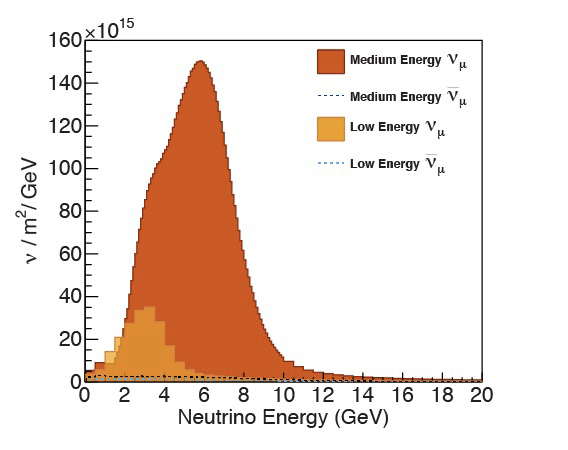
\includegraphics[scale=0.38]{Figures/Chapter2/fluxantineutrino.png}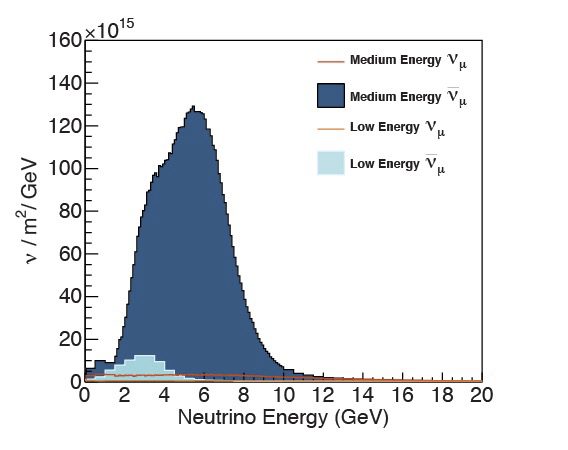
\includegraphics[scale=0.38]{Figures/Chapter2/fluxneutrino.png}
        \caption{Absolute flux for the neutrino mode (left) and the antineutrino mode (right) for the LE and ME eras.} 
\label{fig:MnvExp:NuMI:Flux}
\end{figure}

During the period of 2009 to 2012 the MINER$\nu$A detector collected data in the Low Energy (LE) mode of the NuMI beam, with a $<E_\nu> = 3$ GeV. For the period 2013 to 2019, it collected data in the Medium Energy (ME) mode, with a $<E_\nu> = 6$ GeV.  In the \textbf{Figure} \ref{fig:MnvExp:NuMI:Flux}.



\subsection{NuMI Design}

The NuMI beam uses the proton beam produced by the Fermilab Main Injector with an energy of 120 GeV. The proton beam starts accelerating hydrogen ($H^-$) ions using a radio-frequency quadrupole until 750 KeV. In the second stage, the ions are accelerated by a linac from 750 KeV to 400 MeV. The ions are passed through a thin carbon foil to remove the electrons from the $H^-$ obtaining only protons. 

\begin{figure}[!htb]
\centering
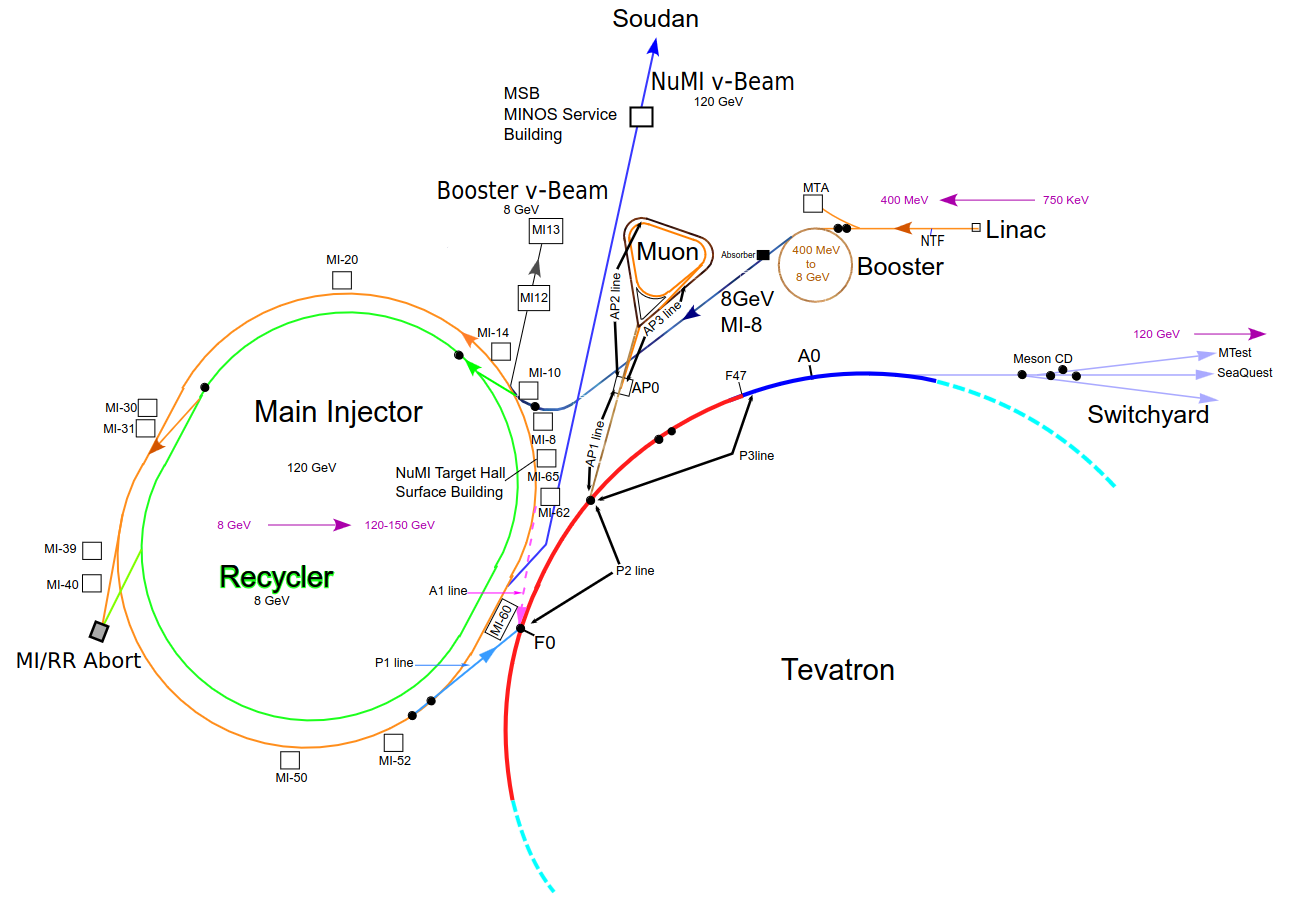
\includegraphics[scale=0.29]{Figures/Chapter2/AcceleratorComplex.png}
        \caption{Schematic of the Fermilab Accelerator complex. Image from \cite{Numi}.} 
\label{fig:MnvExp:NuMI:SchematicMainInjector}
\end{figure}

In the third stage the protons pass to the booster; it is a 75 m radius synchrotron accelerator that accelerates the protons from 400 MeV to 8 MeV, at the same time it groups the protons in 1.6 $\mu s$ long batches. 

The last stage of acceleration is on the Main Injector; it is a proton synchrotron 7 times the circumference of the booster. It accelerates the protons from 8 GeV to 120 GeV of energy. The beam produces is has Gaussian shape with a $\sigma =$ 1.1 mm, with a \textit{Cycle Time} = 1.87 s and 10 $\mu s$ beam spill duration. In the  \textbf{Figure} \ref{fig:MnvExp:NuMI:SchematicMainInjector} all the stages of acceleration are shown.

A portion of the proton spills is used by NuMI to produce the neutrino beam, the beam is bent in direction to the NuMI Target Hall. Here, the protons are steered to a graphite target. The interaction of the protons with the graphite target produces an hadronic shower where the charged hadrons are focused by two parabolic magnetic horns in direction to the decay pipe. Depending of the current orientation of the current in the pipe, the neutrino mode or antineutrino mode beam can be chosen. The major portion of the hadrons produced are pions and kaons, the predominant decay channel for pions is $\pi^+ \longrightarrow \mu^+ + \nu_\mu$ and $K^+ \longrightarrow \mu^+ + \nu_\mu$ giving a $\nu_\mu$ beam; for the case of the antineutrino beam, the negative hadrons are focused, obtaining as a result $\Bar{\nu}_\mu$. 


\begin{figure}[!htb]
\centering
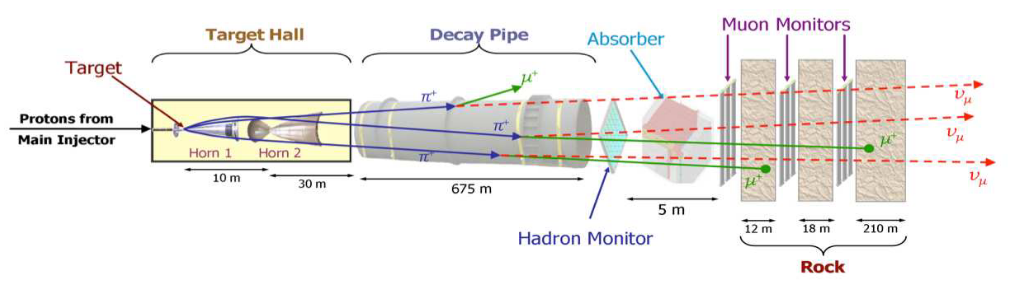
\includegraphics[scale=0.38]{Figures/Chapter2/NuMIScketch.png}
        \caption{Schematic of the Fermilab NuMI Beam. Image from \cite{Numi}.} 
\label{fig:MnvExp:NuMI:SchematicNuMIBeam}
\end{figure}

When the horns focus positive hadrons, the beam consists of 93\% of $\nu_\mu$, 6\% $\Bar{\nu}_\mu$ and 1\% $\nu_e + \Bar{\nu}_e$. In the \textbf{Figure} \ref{fig:MnvExp:NuMI:NuMIBeamComponents} We can observe the different components of the neutrino beam for the neutrino mode in the ME era. 
\begin{figure}[!htb]
\centering
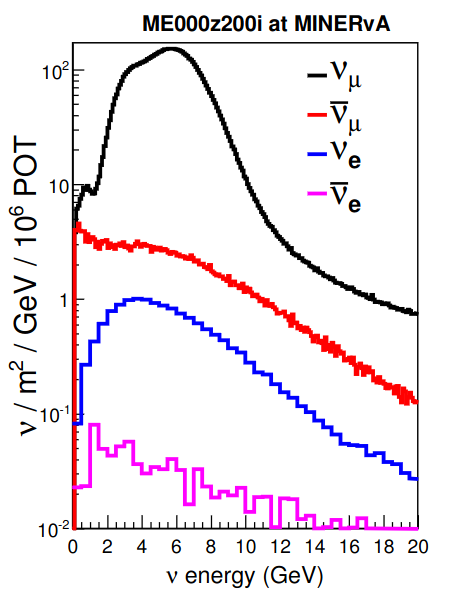
\includegraphics[scale=0.4]{Figures/Chapter2/NuMIbeamComponents.png}
        \caption{Neutrino beam components. Image from \cite{LeoThesis}.} 
\label{fig:MnvExp:NuMI:NuMIBeamComponents}
\end{figure}


\subsubsection{NuMI components}
In this subsection, the components of the NuMI beam are described in more detail as the components of NuMI.

\textit{NuMI Target Hall}

It is a complex that contains the major part of the components that produce the neutrino beam. In addition to containing a large part of the NuMI instrumentation, it has the roll to shield the high levels of radioactivity, heating, and thermal shock that are produced while the beam is on.  

The Target Hall is located in Fermilab approximately 41 m underground, 69 m of length, 8.1 m wide, and 12.5 m high. Initially, the beam was designed with the goal of sending neutrinos to MINOS Near (in Fermilab) and Far (in Soudan Laboratory, Minnesota) detectors; therefore, the neutrino beam is bent $3.343^o$ downward.  

\begin{figure}[!htb]
\centering
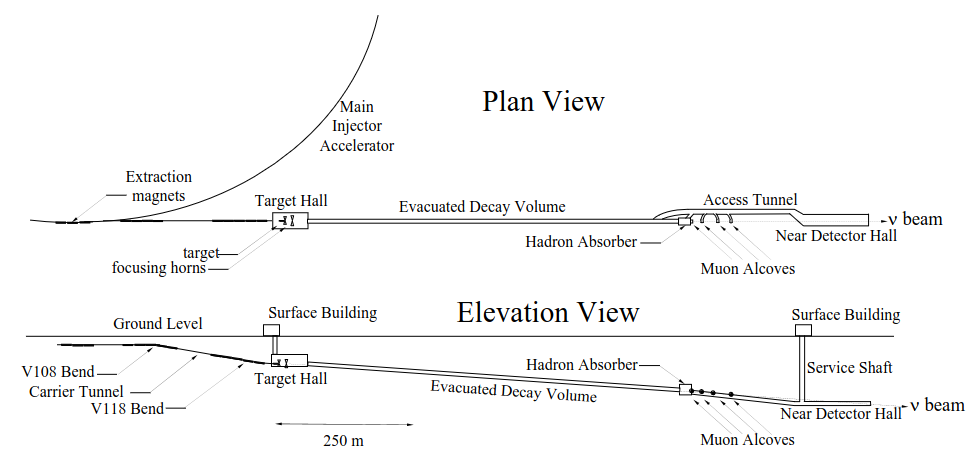
\includegraphics[scale=0.4]{Figures/Chapter2/NuMIFacilityViews.png}
        \caption{Views of the NuMI beam complex. Image from \cite{Numi}.} 
\label{fig:MnvExp:NuMI:NuMIviews}
\end{figure}

The instrumentation in the Target Hall allows us to fix the different beam energy configurations. The energy configuration depends on the distance between the horns and the target, therefore, it is necessary to have a central chase. In this chase the components and instrumentation of the beam can be moved depending on the beam configuration, at the same time the chase is also part of the cooling system. 

The cooling system recirculates air in the different components with a capacity of 240 kW of cooling. This system removes heat for the correct functioning of the beam. For the horns, the cooling system uses water to control the temperature.

The NuMI Target Hall has a crane that allows one to move, repair, and replace equipment remotely. This also has a Work Cell that is a shielded facility where personnel can access and work on the maintenance of the equipment. 

\textit{The NuMI Target}

The NuMI target is designed to support until 400 kW power without disintegrated, at the same time it should produce the maximizing the production of hadrons and reducing the interactions of the hadrons with the target. So, the target can not be very robust because it increases the interaction of the hadrons with the target. The design of the target has to consider that it has to have a high thermal conductivity, it should be available to maintain its mechanical condition under high temperature conditions, withstand long operational journeys and radiation damage. 

The NuMI target is made of graphite of type ZXF-5Q with a density of 1.78 g/cm$^3$ \cite{Numi}. It consists of 48 segments of 24 mm long (in beam direction)$\times$ 63 mm tall $\times$ 7.4 mm wide The total length of the target is 95.38 cm, 0.3 mm apart \cite{BenThesis}.

\begin{figure}[!htb]
\centering
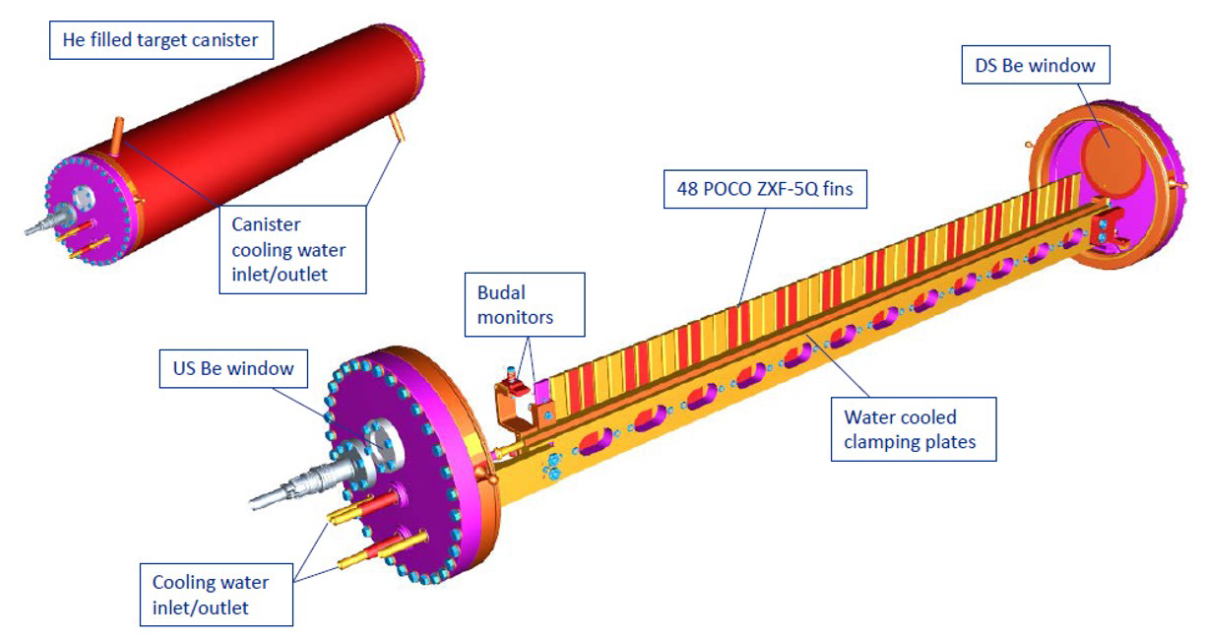
\includegraphics[scale=0.33]{Figures/Chapter2/NuMITarget.png}
        \caption{NuMI Target design for the ME era. Image from \cite{NuMITarget}.} 
\label{fig:MnvExp:NuMI:NuMITarget}
\end{figure}

The NuMI Target is isolated by vacuum and is surrounded by two stainless steel tubes that carry the water coolant. These are counted in an aluminum canister filled with He. The entrance and exit of the target vessel are made of beryllium. Budal monitors \cite{Budal} are used to check the alignment of the target with respect to the beam. 

\textit{The Target/Baffle Carrier}

The Baffle \cite{NOvATDR} protects the neck of the horn and the cooling hardware from miss-steered beam pulses. It consists of a 1.5-long graphite core with 57 mm of diameter encased in an aluminum tube. It has a 13 mm diameter center hole along the rod, where the proton beam passes. 

The target and the baffle are mounted on a structure called \textit{Target/Baffle Carrier}. This brings mechanical support, connections to the cooling system, and connection to the electrical lines. This structure has installed positioning motors that allow the target to move vertically and horizontally. 

 \begin{figure}[!htb]
\centering
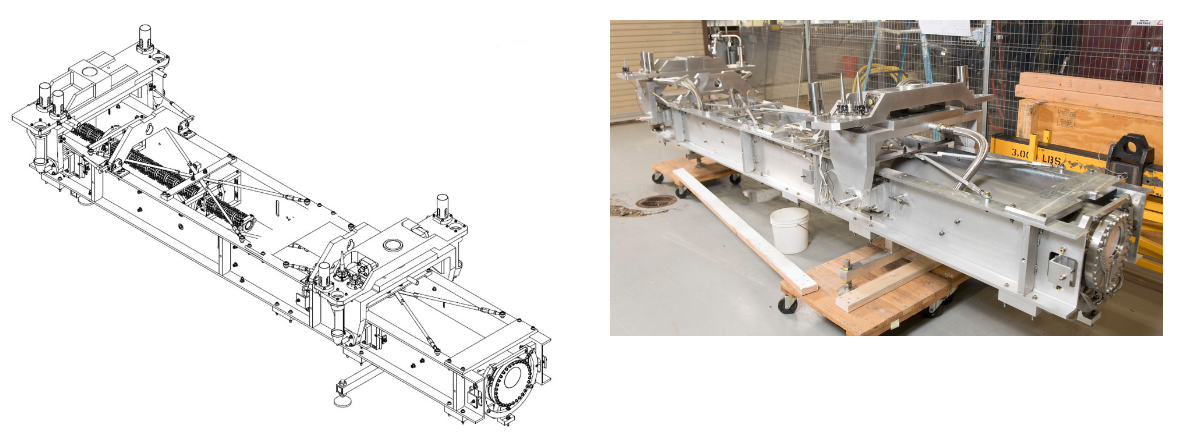
\includegraphics[scale=0.33]{Figures/Chapter2/TargetCarrier.png}
        \caption{Left, NuMI Target/Baffle design. Right, picture of the NuMI Target/Baffle carrier with the target installed. Image from \cite{NuMITarget}.} 
\label{fig:MnvExp:NuMI:NuMITargetCarrier}
\end{figure}

\textit{Magnetic Horns}

The magnetic horns have as their main objective maximize the neutrino flux focusing the secondary particles produced in the target on direction of the detectors, at the same time that can be used to select the neutrino energy spectrum. In the \textbf{Figure} \ref{fig:MnvExp:NuMI:HornsFocusSystem} shows a diagram of how the trajectory of the particles is modified by the horns. 

\begin{figure}[!htb]
\centering
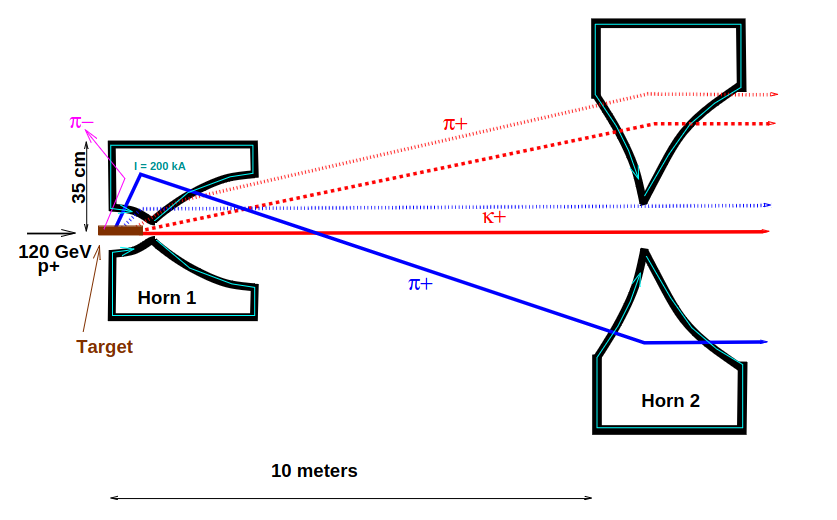
\includegraphics[scale=0.33]{Figures/Chapter2/HornsFocusSystem.png}
        \caption{Schematics of the Horn 1 of Horn 2 modifying the trajectory of the particles. Depending the current direction of the current in the horns the $\nu_\mu$ or $\Bar{\nu}_\mu$ mode can be selected. Image from \cite{Numi}.} 
\label{fig:MnvExp:NuMI:HornsFocusSystem}
\end{figure}

The horns are made of an alloy of nickel-plated aluminum in the inner conductor, and for the outer conductor it uses anodized aluminum. The inner conductor of Horn 1 is 2 mm thick and 3 mm thick for Horn 2 in most regions. The thickness of the horns should be such that it allows the passage of a large electric current and avoids the absorption or interaction of the secondary hadrons with the horns. The double paraboloidal shape of the horns produces a toroidal magnetic field in which the intensity of the magnetic field falls as the inverse of the radium between the inner and the outer conductors. The expected magnetic field in the longitudinal axis of the horns should be zero and in the maximum transverse field 3T. To produce the magnetic field in the horns, a pulsed 200 kA current passes through them with a duration of 2.3 ms.

The high current and the interaction of the hadrons with the horns increase the heat of those, hence, it is necessary to have a cooling system to guarantee a good operation during long periods of time. The cooling system sprays water to the inner conductor keeping the temperature below 100 C. 

\begin{figure}[!htb]
\centering
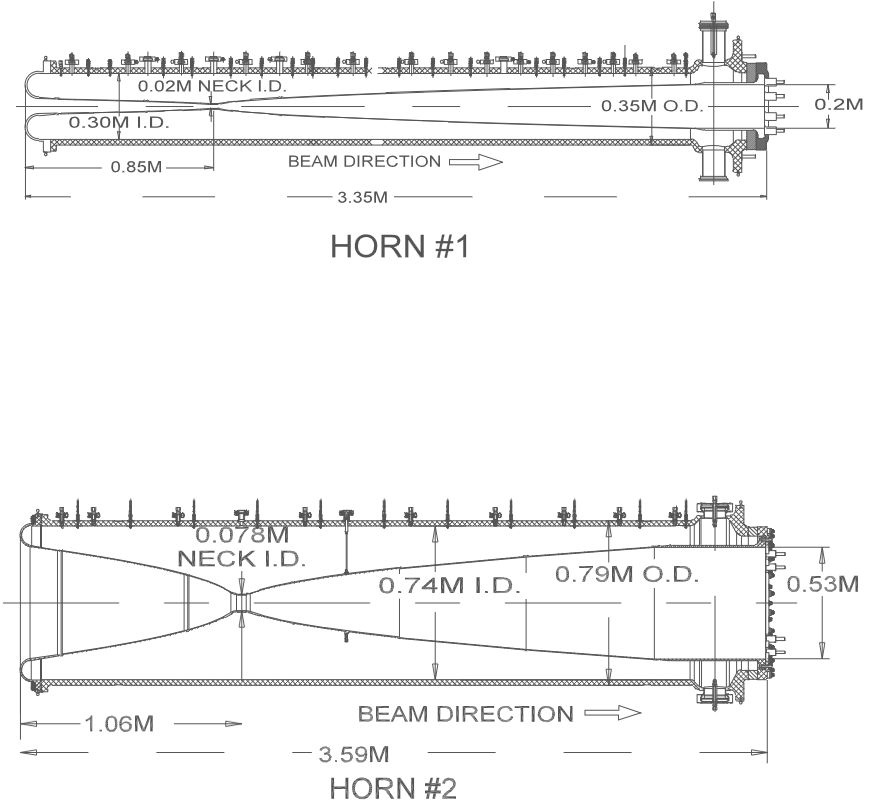
\includegraphics[scale=0.33]{Figures/Chapter2/SchematicMagneticHorns.png}
        \caption{Schematics of the Horn 1 of Horn 2. In the images the dimensions and longitudinal cut of the horns are shown. Image from \cite{Numi}.} 
\label{fig:MnvExp:NuMI:NuMIHornsSchematic}
\end{figure}

Depending of the momentum and the charge of the hadrons, the effects of the horns on the hadrons can be categorized as follows:

\begin{itemize}
    \item \textit{Deflected}: Selecting the direction of the current, the horns can be used to focus only positive or negative hadrons. This allows to select between $\nu$ or $\Bar{\nu}$ beam. It means that when the $\nu$ mode is selected, the negative particles are deflected by the horns, and vise-versa.
    \item \textit{Unfocused} : These are the hadrons that pass very close to the necks of the horns and the trajectory of this particles is not modified by the horns. The most part of these are hadrons with a momentum above to 15 GeV. 
    \item \textit{Underfocused} : These are hadrons that have to pass by the two horns to be focused. The range of the momentum for the hadrons is between 5 GeV and 15 GeV.
    \item \textit{Overfocused}: These are particles that pass throughout the horn 1 and horn 2. Unlike of the underfocused, these are hadrons with a momentum below to the 5 GeV. 
    \item \textit{Horn-1-only}: These are particles that are corrected only by the Horn 1 and that pass throughout the neck of the Horn 2. The transversal momentum of these hadrons usually is above to the 0.2 GeV.
    \item \textit{Horn-2-only} : These are hadrons that pass throughout the neck of the Horn 1 and that are only corrected by the Horn 2. The momentum of these hadrons is between the range of 9 GeV and 15 GeV.
\end{itemize}

\begin{figure}[!htb]
\centering
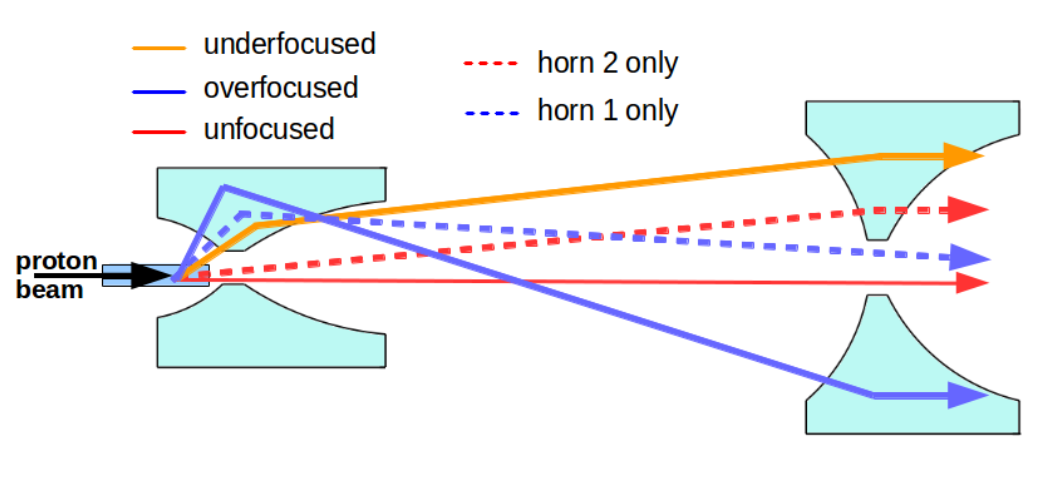
\includegraphics[scale=0.33]{Figures/Chapter2/FocusingComponents.png}
        \caption{Image where the categories of focusing effects are represented. Image from \cite{LeoThesis}.} 
\label{fig:MnvExp:NuMI:NuMIFocusingComponents}
\end{figure}

The focused hadrons with the largest momentum are the hadrons that have a small component of the transversal momentum with respect to the proton beam. Therefore, if the horns are close, the number of focused hadrons with low momentum increases with respect to the high momentum, and vise versa. Considering this fact, the distance between the horns can be used to select the spectrum energy of the focused hadrons, resulting in a selection of the spectrum of the neutrino beam. The NuMI beam can be used in three energy configurations. Low Energy (LE) where the $<E_\nu>=3.5$ $GeV$, Medium Energy (ME) where $<E_\nu>=7$ $GeV$ and High Energy where the $<E_\nu> = 14$ $GeV$\cite{BeamOptics}. 

\begin{figure}[!htb]
\centering
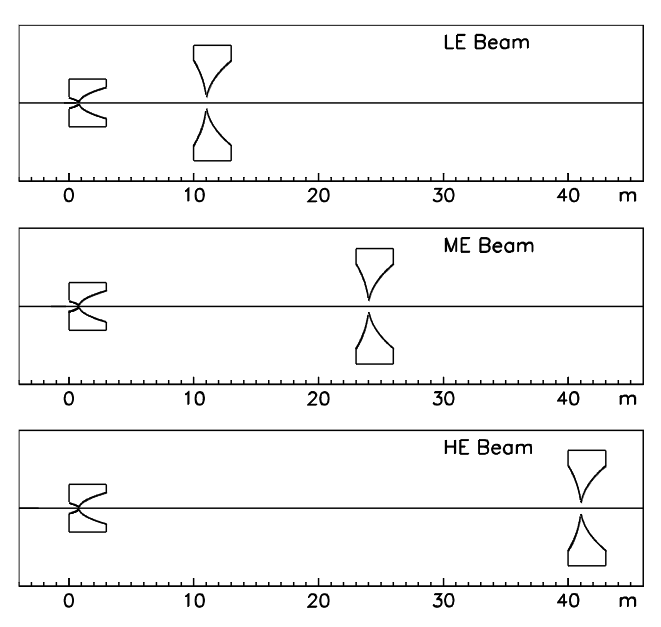
\includegraphics[scale=0.4]{Figures/Chapter2/HornsDistance.png}
        \caption{In this image the distance between the horns for the different energy configurations is shown. Image from \cite{BeamOptics}.} 
\label{fig:MnvExp:NuMI:NuMIHornDistance}
\end{figure}

\begin{figure}[!htb]
\centering
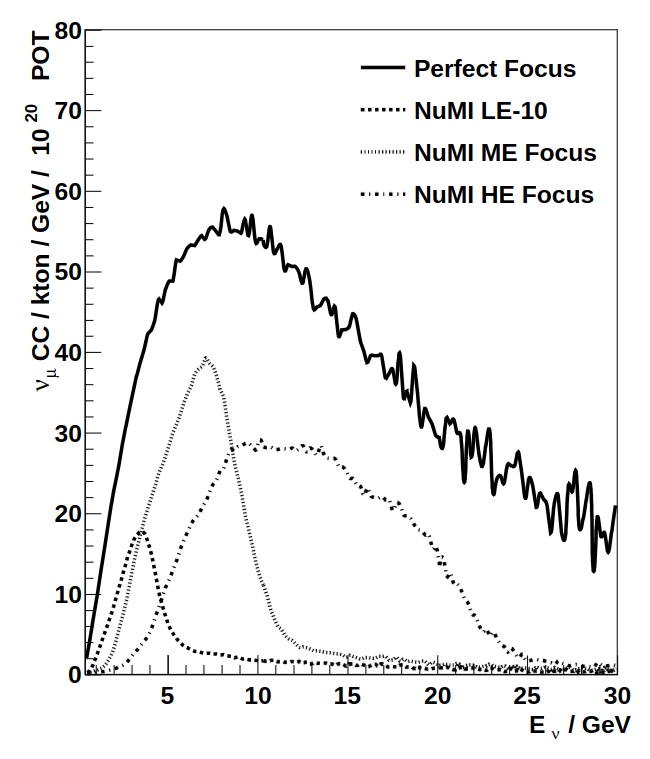
\includegraphics[scale=0.3]{Figures/Chapter2/nuAllSpectrums.png}
        \caption{In this graph, the simulated neutrino spectrum for the different neutrino neutrino energy beam configurations. Image from \cite{Numi}.} 
\label{fig:MnvExp:NuMI:Neutrino spectrum}
\end{figure}

\textit{Decay Pipe}

After to focus the secondary hadrons, these pass through the \textit{Decay Pipe}. Here, most of the hadrons decay and produce the neutrino beam. The goal of the Decay Pipe is to reduce the interactions of the hadrons with the surroundings. To reduce the interactions inside of the Decay Pipe is produced conditions of a low density environment. 

The dimensions of the Decay Pipe are 2 m in radius $\times$ 645 m in length. It is surrounded by concrete to reduce the radiation effects in groundwater. The Decay Pipe is designed to work under internal vacuum conditions and with other low density gases such as helium. 

The collisions of particles with the pipe heat the structure; with the aim to reduce the temperature and to guarantee long operations of the facility, a cooling system is installed in the pipe. This allows us to keep a temperature below the 50 C. 

\textit{Absorber}

Downstream of the Decay Pipe, a structure of aluminum, steel, and concrete is installed to stop protons that did not interact with the NuMI Target and other remnant beam particles; this structure is the absorber. The absorber is an essential component to reduce the levels of radiation and to avoid the groundwater from radiation. The deposition of the energy of the particles generates a temperature increment of the absorber, hence this has a cooling system to maintain the temperature below to 50 C. 

\textit{Muon Shield} 

The Muons shield is the last part of the NuMI beam; this works as a shield for the detectors situated in the MINOS Hall from the muons produced in the decay of the mesons in the production of the neutrino beam. This consists of 240 m of dolomite rock that stops the muons. 

\pagebreak



\section{MINER$\nu$A Detector}
\label{Cap:MnvExp:MnvDetector}

The Minerva detector is a fine-grained detector that uses plastic scintillators as active detection material to reconstruct the trajectory and energy of the charged particles produced in neutrino interactions. The design of the detector allows one to make a 3D spatial reconstruction at the same time that allows to make a reconstruction of the deposited energy by calorimetric and range techniques. 

The MINER$\nu$A experiment physics goals include producing the measurement of the inclusive and exclusive cross section studies of diverse types of interactions; therefore a good energy reconstruction for low and high energy Final States Interaction (FSI), particle identification and the understanding of multiple interactions in a single beam spill are necessary. Considering the previous points, the detector was designed to use different passive nuclear targets, having as active detection material a plastic scintillator, the fact that it is a low density active detection material that allows a good reconstruction of low energy events. A large portion of the detector is filled with this material with the aim of reconstructing the multiparticle final state at the same time, which is surrounded by electromagnetic (ECAL) and hadronic (HCAL) calorimeters to contain all the particles generated in the interaction. The muons are particles that are not easy to stop; for this reason the detector was situated upstream of the MINOS Near detector with the aim of using it to reconstruct the momentum and determine the charge of the muons produced in the neutrino interactions inside of MINER$\nu$A.


\begin{figure}[!htb]
\centering
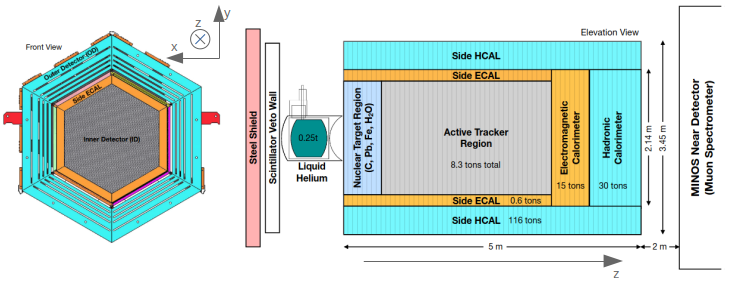
\includegraphics[scale=0.5]{Figures/Chapter2/DetectorScheme.png}

        \caption{Scheme of the MINER$\nu$A detector. . Figure from \cite{MINERvA}} 
\label{fig:MnvExp:MnvDetector:Scheme}
\end{figure}

The MINER$\nu$A coordinate system is set as follows. The origin of the plane X-Y is in the center of the MINER$\nu$A hexagon. The Z axis origin is situated 1200 cm downstream of the MINOS detector, this goes along the center of the MINER$\nu$A detector. The direction of the neutrino beam point 3.34$^o$ downward in the Y-Z plane. 

In the transversal direction of the detector it is segmented in the Inner Detector (ID), where the active tracking planes, nuclear targets, downstream Electromagnetic Calorimeter (ECAL), and the Hadronic Calorimeter (HCAL); and the Outer Detector (OD) consists of a steel frame with plastic scintillator embedded that works as HCAL and mechanical support to the planes.   

\subsection{Active Tracking planes}
\label{Cap:MnvExp:MnvDetector:ActiveTrackingPlanes}

The detector has active and passive nuclear targets. Active nuclear targets are triangular plastic scintillator strips. When a charge particle passes through a scintillator materials, the particle transfers part of its energy to the material; after a short time it becomes de-energized emitting a pulse of light\cite{DetectionTechniques}. 

The triangular scintillator stripes have a base of 3.3 cm and 1.7 cm height, the length of the strips varies between 85 cm and 170 cm. These are made up of polystyrene doped with 2,5-diphenyloxazol (PPO) and 1,4-bis(5-phenyloxazol-2-yl) benzene (POPOP). These two materials work as weave length shifters. The polystyrene emits light in the far UV region, the PPO absorbs the light and re-emits it in the region of the near UV, and then the POPOP absorbs this light and emits it as visible blue light. Along of center of the scintillator strips there is placed an optical fiber that absorbs the blue light, and then this re-emits the light on green in the ends of the fiber. The reason why the light has to be shifted is because the photo-detectors that transform the light to electrical signals work more efficiently with green light; this process is explained in more detail in \textbf{section} \ref{Cap:MnvExp:MnvDetector:PhotoDetectionSystem}. The scintillator strips are painted with white EJ-510 $TiO_2$ Eljen paint\cite{StripsPaint}. 


\begin{figure}[!htb]
\centering
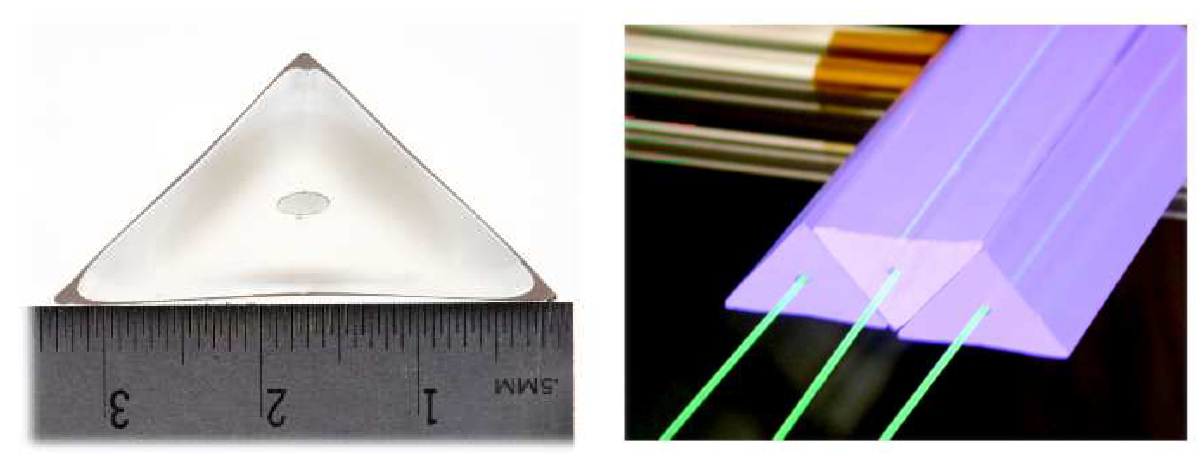
\includegraphics[scale=0.3]{Figures/Chapter2/ScintStripes.png}

        \caption{Images where the plastics scintillators are shown. Figure from \cite{MINERvA}} 
\label{fig:MnvExp:MnvDetector:TriangularStripes}
\end{figure}

The scintillator strips are arranged as is observed in the \textbf{Figure} \ref{fig:MnvExp:MnvDetector:StripsArrange}. The tracking planes are made up of two plastic scintillator planes. In each plane there are 127 strips glued using 3M-DP190 translucent epoxy. The planes are also optically insulated from the exterior. 

\begin{figure}[!htb]
\centering
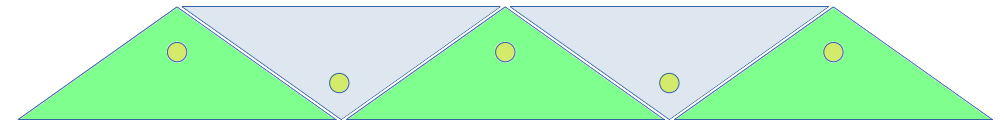
\includegraphics[scale=0.3]{Figures/Chapter2/stripsArrange.png}

        \caption{Scheme that shows how are arranged the scintillator strips to compose the tracking planes.} 
\label{fig:MnvExp:MnvDetector:StripsArrange}
\end{figure}

The tracking planes can be oriented 1 of X, U or V configuration. The orientation of the strips in the X configuration is $90^o$ with respect to the horizontal orientation. For U and V are rotated $60^o$ and $-60^o$, respectively, taking as reference the X orientation, in the \textbf{Figure} \ref{fig:MnvExp:MnvDetector:PlanesOrientations} three schemes of orientation configurations are shown. The three orientations are used to avoid reconstruction ambiguities for events that contain two particles and deposit energy in orthogonal planes. For the shape and the arrangement of the scintillator strips in the tracking planes, each time that a charge particle passes throughout a plane, most part of the particles will interact with two scintillator strips. 

\begin{figure}[!htb]
\centering
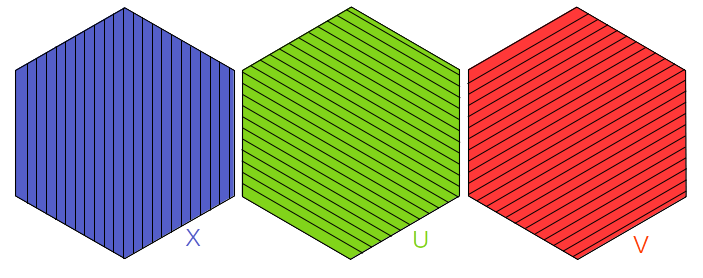
\includegraphics[scale=0.4]{Figures/Chapter2/PlanesOrientation.png}

        \caption{Scheme with that shows the different tracking modules orientations.} 
\label{fig:MnvExp:MnvDetector:PlanesOrientations}
\end{figure}

The planes are grouped in tracking modules; these consist of two tracking planes XU or XV. The modules are stacked in the pattern XUXV, this arrange allows a 3D reconstruction of the charged particles produced by the neutrino interactions that pass through the detector. In the \textbf{Figure} \ref{fig:MnvExp:MnvDetector:TrackingModules} shows a representation of charged particles passing through the tracking modules. 

\begin{figure}[!htb]
\centering
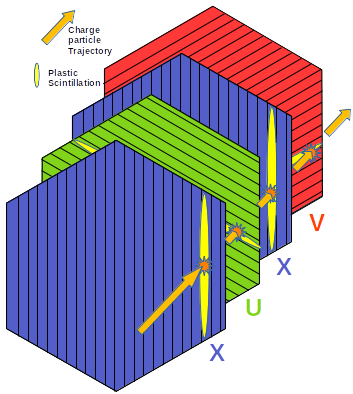
\includegraphics[scale=0.5]{Figures/Chapter2/TrackingModules.png}

        \caption{Scheme where the arrangement of the tracking modules is shown. In the figure is represented how a charged particle produce a signals in the planes.} 
\label{fig:MnvExp:MnvDetector:TrackingModules}
\end{figure}

All the planes are rounded by hexagonal lead frames that play the role of ECAL. They are framed by a steel hexagonal frame that brings mechanical support to the hole plane, and it is an HCAL. The ECAL and the HCAL that rounds the tracking planes are shown in the \textbf{Figure} \ref{fig:MnvExp:MnvDetector:Scheme}.

\subsection{MINERvA detector Regions}
\label{Cap:MnvExp:MnvDetector:MnvDetectorRegions} 

\begin{itemize}
    \item \textit{Veto wall}

    The Veto Wall is located upstream of the MINER$\nu$ A detector, consisting of a steel plate of 5 cm of thickness followed by a plate of plastic scintillator. This section of the detector is used to detect muons that are produced by the interaction of the neutrino beam with the dolomite rock of the muon absorber. These muons are commonly called \textit{rock muons}.

    \item \textit{Nuclear Targets Region}

    The nuclear target region is made up of active and passive targets. The passive materials are Liquid Helium ($He$), Carbon ($C$), Lead ($Pb$), Water ($H_2O$) and Steel ($Fe$). In the \textbf{Figure} \ref{fig:MnvExp:MnvDetector:TargetRegion} the order in which the planes were placed for passive and active materials in the target region is shown. The C, Pb, $H_2O$ and Fe targets ,in the same way as the active tracking planes, are supported by the ECAL and HCAL.
    
    \begin{figure}[!htb]
    \centering
    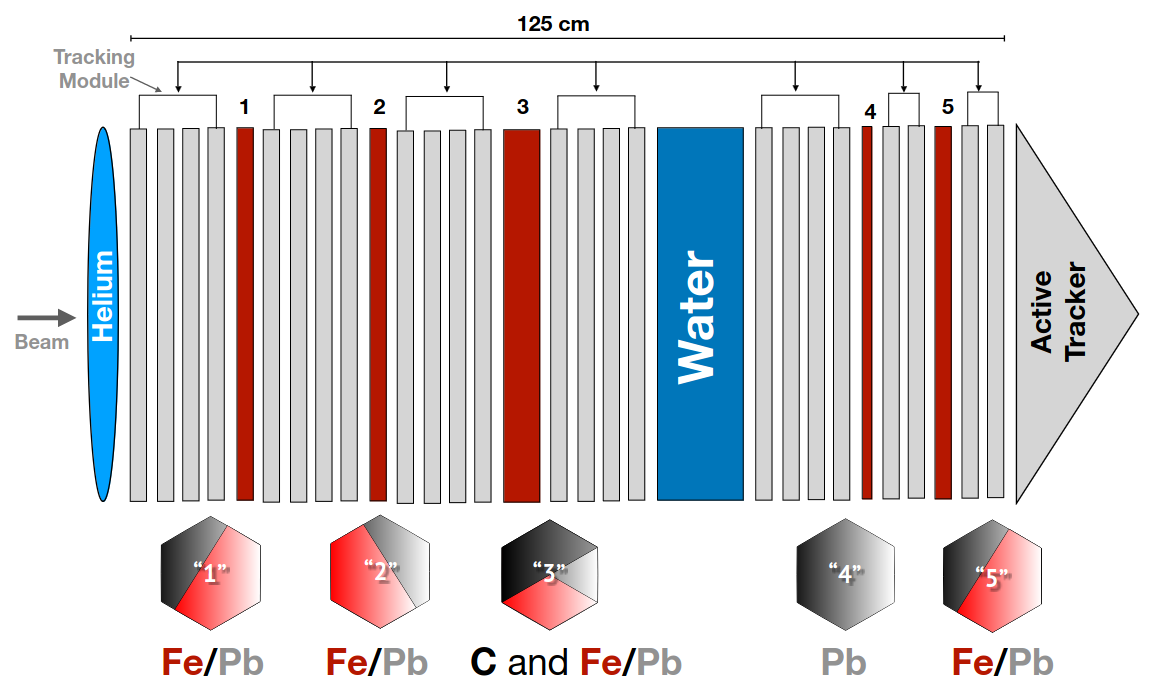
\includegraphics[scale=0.35]{Figures/Chapter2/TargetRegion1.png}

        \caption{Scheme that shows the order that are arranged the target planes in the Target Region. The target region is composed for a cryostat with the Liquid He target, 5 solid targets and the water target. Figure from \cite{MarvinThesis}} 
    \label{fig:MnvExp:MnvDetector:TargetRegion}
    \end{figure}
    
    The He target cryostat is located downstream from the veto wall. This target is capable of containing 2300 L of liquid He, it was filled during the last parts of the run \cite{MINERvA}. The other targets are located upstream of the He target. With the aim to localize the neutrino interaction vertex, the nuclear targets planes are located between tracking modules, as shown in the \textbf{Figure} \ref{fig:MnvExp:MnvDetector:TargetRegion}, except for the thin lead target, where only 1 tracking module is located upstream. After the fifth target, the modules of the tracker region start. In the \textbf{Tables} the information about the composition of the targets is described. 

    \begin{table}[!htb]
        \centering
        \begin{tabular}{c c c c c c c c}
            \textbf{Material} & \textbf{Density} & \textbf{C(\%)} & \textbf{Si (\%)} & \textbf{Mn (\%)} & \textbf{Fe (\%)} & \textbf{Cu (\%)} & \textbf{Pb (\%)} \\ 
             & \textbf{(g/cm$^2$)} & & & & & & \\ \hline
            Steel & 7.83±0.03 & 0.13 & 0.2 & 1.0 & 98.7 & - & - \\
            Lead & 11.29±0.03 & - & - & - & - & 0.05 & 99.95\\
            Graphite & 1.74±0.01 & >99.5 & - & - & - & - & - \\ \hline
        \end{tabular}
        \caption{In this table the density and element composition for the solid nuclear targets is shown. Table from \cite{MINERvA}}.
        \label{tab:Chapter2:Detector:NuclearTargetsComposition}
    \end{table}

    \begin{table}[!htb]
        \centering
        \begin{tabular}{c c c c c c}
            \textbf{Target} & \textbf{z-location} & \textbf{Thickness} & \textbf{Fiducial area} & \textbf{Fiducial mass} & \textbf{Total mass}  \\ 
             & \textbf{(cm)} & \textbf{(cm)} & \textbf{cm$^2$} & \textbf{(kg)} & \textbf{(kg)} \\ \hline
            1-Fe & 452.5 & 2.567±0.006 & 15999 & 322 & 492 \\ 
            1-Pb & 452.5 & 2.578±0.012 & 9029 & 263 & 437 \\
            2-Fe & 470.2 & 2.563±0.006 & 15999 & 321 & 492 \\ 
            2-Pb & 470.2 & 	2.581±0.016 & 9029 & 263 & 437 \\
            3-Fe & 492.3 & 	2.573±0.004 & 7858 & 158 & 238 \\ 
            3-Pb & 492.3 & 2.563±0.004 & 3694 & 107 & 170 \\
            3-C & 492.3 & 7.620±0.005 & 12027 & 160 & 258 \\ 
            Water & 528.4 & 17–24 & 25028 & 452 & 627 \\
            4-Pb & 564.5 & 0.795±0.005 & 25028 & 225 & 340 \\
            5-Fe & 577.8 & 1.289±0.006 & 15999 & 162 & 227 \\ 
            5-Pb & 577.8 & 1.317±0.007 & 9029 & 134 & 204 \\ \hline
        \end{tabular}
        \caption{The z position, thickness, fiducial area, fiducial mass and total mass of the nuclear targets are shown. The z-location is determined according to the coordinate system described in the text. Table from \cite{MINERvA}. }
        \label{tab:Chapter2:Detector:Sizes}
    \end{table}

    The water target, unlike the solid targets, is held by a circular frame. The diameter of this frame is larger than that of the MINER$\nu$A inner detector size. The water container is made of two Kevlar\textsuperscript \textregistered sheets. The internal hydrostatic pressure of the water deforms the shape of the water container, and for that reason the water target is not well defined. The geometry of the targets is part of the parameters of the particle simulation, and it is necessary to have a good approximation of the shape of the targets, with the aim of obtaining the best approximation to the water target shape; the container shape was simulated via finite element analysis. 

    \begin{figure}[!htb]
        \centering
        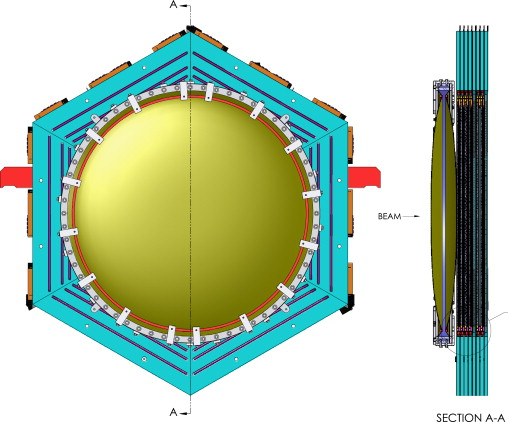
\includegraphics[scale=0.6]{Figures/Chapter2/WaterTarget.jpg}
        \caption{Scheme of the water target. Image from \cite{MINERvA}.}
        \label{fig:MnvExp:MnvDetector:WaterTarget}
    \end{figure}

    
    \item \textit{Active Tracker Region}
    
    The active tracker region consists of 61 tracker modules, giving a total of 122 tracking planes. In this region the ID volume is completely filled with plastic scintillator, described in \ref{Cap:MnvExp:MnvDetector:ActiveTrackingPlanes}, and the OD volume consists of the ECAL and HCAL.
    
    \item \textit{Electromagnetic and Hadronic Calorimeter modules}
    
    The ID ECAL is located upstream of the tracker region. The configuration of the planes in the ECAL region is similar to the tracker region, except that each plane has a 0.2 cm thick layer of lead embedded on the upstream side of the plane. This layer helps to stop the electrons and photons produced in the interaction vertex, obtaining a good energy resolution and directional information. This region contains 10 of these modules. 

    For the case of the ID HCAL, it has a similar configuration to the tracker region, but it has an steel plane of 2.54 cm thick, each two planes, that is, each module has one steel plane. In the same way that the ECAL but with heavier particles, it allows a good energy resolution and directional information of particles such as protons and neutrons. 
    
\end{itemize}

\subsection{MINOS Near Detector}
\label{Cap:MnvExp:MnvDetector:MINOS}

The MINER$\nu$A detector is situated 2.1 m from the MINOS detector and is used by MINER$\nu$A as a muon spectrometer. The MINOS Near detector is designed to measure the muon neutrino flux close to the NuMI beam, performing a precise measurement of the neutrino oscillation parameters for the muon neutrino disappearance. The MINOS Near detector is a magnetized tracking calorimeter composed of planes of plastic scintillator and iron that give a total mass of 1 kTon \cite{MINOSpaper}. The rectangular coil produces a toroidal magnetic field of average strength of 1.3 T.

\begin{figure}
    \centering
    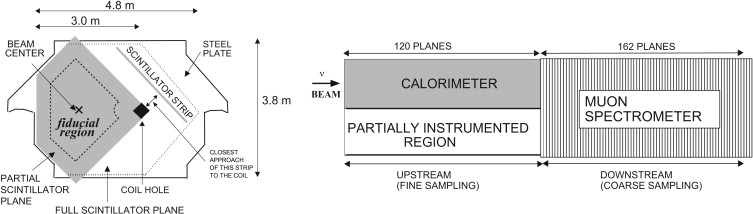
\includegraphics[scale=0.9]{Figures/Chapter2/MINOSNDScheme.jpg}
    \caption{Scheme of the lateral and frontal view of the MINOS Near detector. Some of the main components of the detector are shown. Figure from \cite{MINERvA}.}
    \label{fig:MnvExp:MnvDetector:SchemeMINOSND}
\end{figure}

The MINOS detector can measure the energy of the muon by the curvature or by range. Reconstruction by range is applied when the muon is contained in the detector, measuring the ionization energy in the plastic scintillator and adding the correction for the passive steel. For the cases where the muon is not contained in the detector, the energy is reconstructed by the curvature of the track of the muon deflected by the magnetic field in MINOS. The energy measured by range is more precise that by curvature, for that it is preferred in the case that it is reconstructed by the two methods. For reconstruction of the total muon energy, the energy measured by MINOS is added to the deposited energy of the muon in MINER$\nu$A. 


\begin{figure}[!htb]
    \centering
    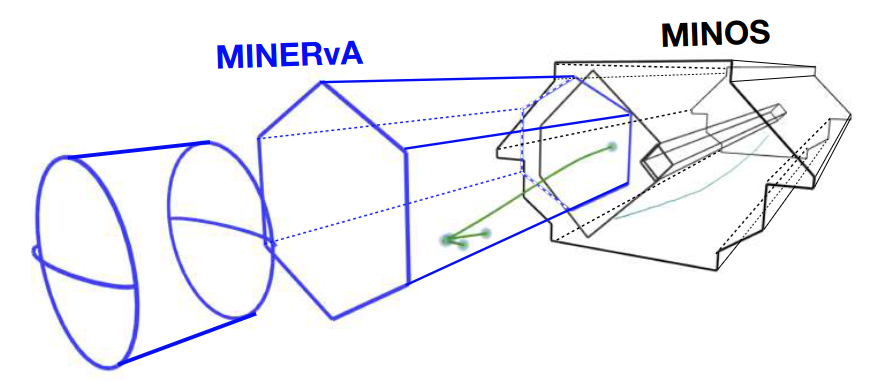
\includegraphics[scale=0.4]{Figures/Chapter2/MnvMINOS.png}
    \caption{Scheme that shows the volume of the He target, ID volume and the MINOS detector. In the scheme is shown how the MINER$\nu$A detector is aligned to the fiducial region of the MINOS detector. Image from \cite{MarvinThesis}.}
    \label{fig:MnvExp:MnvDetector:WholeMINERvADet}
\end{figure}

\subsection{Photodetection System}
\label{Cap:MnvExp:MnvDetector:PhotoDetectionSystem}

The light produced in the scintillator is downshifted by a wavelength shifting (WLS) fiber that is located in the center of the scintillator strip. The end of this fiber is polished to a mirror level. The ends of the cables are encrusted to optical connectors from Fujikura-DDK \cite{OpticalConnector}. Each connector holds eight fibers in a linear shape. The connectors are referred to the other DDK connector, this connector holds 8 clear polished fibers. These cables transmit light from the WLS to the photomultiplier (PMT) boxes. All WSLs were tested for attenuation at different distances of the fiber. For clear fibers, they were tested for the transmission of light. These procedures are described in \cite{MINERvA}.

\begin{figure}[!htb]
    \centering
    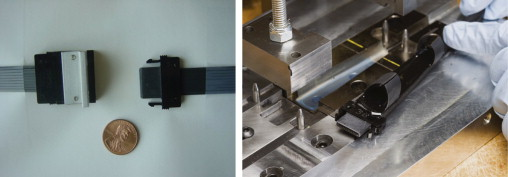
\includegraphics{Figures/Chapter2/OpticCablesConnectors.jpg}
    \caption{In the left, picture of the DDK connector. In the right the process of attach of the optical wires to the DDK connectors. Figure from \cite{MINERvA}.}
    \label{fig:MnvExp:MnvDetector:DDKConnector}
\end{figure}

The optical box consists of a frame that contains the Fiber-end Face plate, the cookie, the PMT, the FEB connector board, two inputs for the Light Injection (LI) system, connecting cables, and the Optical Decoder Unit (ODU). The ODU is an array that connects the Fiber-end face plate to the PMT. In the \textbf{Figure} \ref{fig:MnvExp:MnvDetector:OpticalBox} the components of the optical box are shown. 

\begin{figure}[!htb]
    \centering
    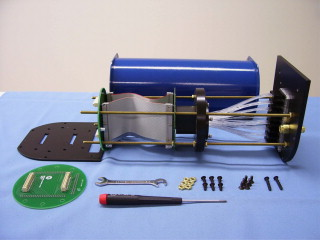
\includegraphics{Figures/Chapter2/OpticaBox.jpg}
    \caption{Picture where the internal components of the optical box. Figure from \cite{MINERvA}.}
    \label{fig:MnvExp:MnvDetector:OpticalBox}
\end{figure}

Photomultipliers, more commonly known as PMTs, are sensitive light detectors that transform the light that is collected by the sensitive region into an electric signal. The physics beyond the PMT is based on the photoelectric effect, when the photons pass through the input window and interact with a cathode it produces photoelectrons, these are accelerated by an electric field produced by a dynodes chain where the electrons collide producing a positive gain in the number of electrons. This technology allows to have information of the initial number of photons given the multiplicative factor of charge, and the size of the signal is related with the deposited energy of the particles on the scintillator. 

\begin{figure}[!htb]
    \centering
    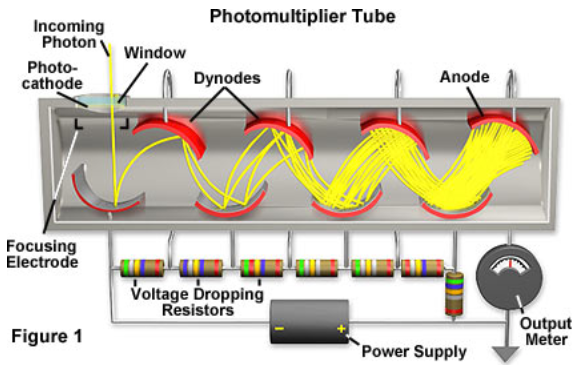
\includegraphics[scale=0.5]{Figures/Chapter2/PMT.png}
    \caption{Scheme where the functionality of a PMT is shown. In the image the mainly components of a PMT are shown. Figure from \cite{PMTHamamatsu}.}
    \label{fig:MnvExp:MnvDetector:PMTfunctionality}
\end{figure}



The PMT model used is H8804MOD-2 manufactured by Hamamatsu Photonics \cite{hamamatsu2007photomultiplier}. The H8804MOD-2 PMT has an 8$\times$8 matrix of 2 mm $\times$ 2 mm pixels, giving a total of 64 pixels. The required quantum efficiency is 12\% at 520 nm and a maximum to minimum pixel gain. The spectral response of the PMT is 300-650 nm.    

The ODU has as main goal to separate physically the signal from adjacent scintillator strips, in the way that these are not adjacent pixels in the PMT. This distribution helps to reduce the crosstalk effects that can be presented in plastic bars. In the \textbf{Figure} \ref{fig:MnvExp:MnvDetector:ODU} a diagram of the fiber pattern is shown. 

\begin{figure}[!htb]
    \centering
    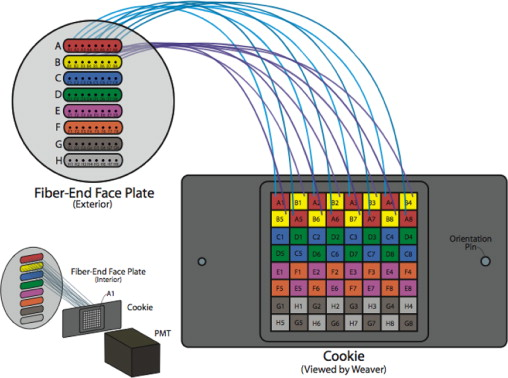
\includegraphics{Figures/Chapter2/ODU.jpg}
    \caption{Pattern of distribution of the fibers for each PMT. Figure from \cite{MINERvA}.}
    \label{fig:MnvExp:MnvDetector:ODU}
\end{figure}

Each optical box has two inputs for the light injection system (LI). This system consists in a light box that produces a blue pulsed light that is sent by two clear optical cables to each optical box, inside the optical boxes the light is distributed uniformly over all the PMT pixels. The LI system turns on during the ones after each beam spill. In this test, the gain of the PMTs is measured and monitored. This procedure is made dearly. 

The output of the PMTs is connected to an electronic board known as the front-end board (FEB). This electronic board digitizes the analog signal's height and timing pulses that come from the PMTs, provides high voltage (HV) to the PMT, and sends the digitized information to the Data Acquisition System (DAQ). 

\begin{figure}
    \centering
    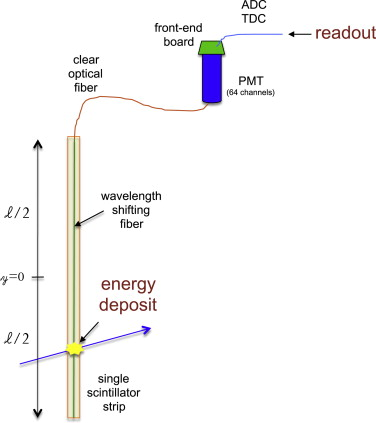
\includegraphics{Figures/Chapter2/OpticalSystem.jpg}
    \caption{Scheme that shows the mainly components of the optical system. It shows how the light travels from the plastic scintillator strips to the optical box. Figure from \cite{MINERvA}.}
    \label{fig:MnvExp:MnvDetector:OpticalSystem}
\end{figure}

\subsection{Data Acquisition System }
\label{Cap:MnvExp:MnvDetector:DAQ}

The Data Acquisition System has a main roll collect all the information generated in the neutrino interaction and save it. After that, the light is produced in the plastic scintillator strips, is explained in the \textbf{Subsection} \ref{Cap:MnvExp:MnvDetector:ActiveTrackingPlanes}, the light is carried by the optical cables to the optical boxes, where the light is transformed into an electrical signal by the PMTs. This signal is passed to an FEB that has six Application Specific Integrated Circuit (ASiC) chips (TriP-t chips)\cite{osti_1012682} controlled by a Field Programmable Gate Array (FPGA) used to digitize the analog signal from the PMTs and store the information. Each PMT sent the information of 64 channels to one FEB, then this FEB is connected to a readout chain that is communicated to a VME\cite{VMEModule} module called Chain Read Out Controller (CROC). A chain had no more than 10 FEBs connected. The CROCs received the timing and trigger signal from the CROC Interface Module (CRIM), which is synchronized to the FNAL Main Injector. Each neutrino beam spill has a duration of 10 $\mu$s and the readout system captures information from the detector during 16 $\mu$s, it starts to take data 0.5 $\mu$s before the neutrino spill arrives and 5.5 $\mu$s after the neutrino spill passes throughout the detector. This time of 16 $\mu$ s is denoted a time gate. At the end of the gate, the readout system collects the data to the readout computer for the archival and monitoring process.

When a particle produces scintillation in a plastic strip, the information about this event is stored as \textit{hits}. These hits are localized by a timestamp relative to the start of a gate. To be considered a hit, all signals must pass a fixed threshold for each discriminator. If the signal passes the threshold, the total signal is integrated and this integrated signal is correlated to the energy deposited by the particle in the strip. Each timestamp has a time resolution of 2.35 ns. 

A detailed description of the DAQ is given in \cite{DAQPERDUE2012179}.

\subsection{Calibration}
\label{Cap:MnvExp:MnvDetector:Calibration}

The calibration of the detector consists of a series of procedures used to convert raw analog-to-digital conversion (ADC) information and convert it on energy hits. The energy hits gives the energy deposited by the particle in the scintillator strip. 



The ADC takes the analog signal that comes from the PMT and transforms it into a digital signal. To measure the deposited energy of the particle in the strip, there are three effects that must be considered from the ADC. The effects are as follows.

\begin{itemize}
    \item Photons attenuation for their travel in the weight light shifting fiber until the end of the plastic strip. 
    \item Photons attenuation for their travel in the clear optical fibers.
    \item The PMT gain per photo-electron produced for the multiplicative effect in the PMT. 
    \item The ADC conversion process. 
\end{itemize}

Considering that the effects described above are the most significant, the following expression is used to measure the energy deposited per particle on the scintillator strip \textit{i}: 

\begin{equation}
    E_i(t) = (ADC_i(t) - Ped_i(t)) \times \frac{FEB_i \times \eta^{Atten}_i \times S_i(t) \times C(t)}{G_i(t)},
    \label{eq:DepositedEnergy}
\end{equation}

where $Ped$ is the noise pedestal for the PMT, the $FEB$ is the ACD conversion gain factor used, $\eta^{atten}$ is the photon attenuation due to the strip, $S$ is the correction factor for each strip, $C$ is the overall time dependent energy scale constant for the whole detector and $G$ is the gain from the PMT.

\subsubsection{Ex situ calibrations}
\label{Cap:MnvExp:MnvDetector:Calibration:ExSitu}
The ex situ calibration is related to all measurements made before the detector is assembled. These were made to have information about the components of the detector; this information is used to make the energy reconstruction. 

The ex situ calibrations are:

\begin{itemize}
    \item \textbf{Module mapper:} The goal of this calibration consist in to measure the photons attenuation in the plastic scintillator and the connections between the optical fibers. The measurements were made using a scanner with a $^{137}Cs$ radioactive source measuring how the lignt was attenuated for different positions in the plane for each strip. This information is used latter to make corrections using the tracking algorithm to determine the attenuation depending the position where the particle pass.
    \item \textbf{PMT testing:} In this test is determined the efficiency, linearity, pixel-to-pixel gain variations, dark noise and cross talk. This test is made before to install the PMT in the optical boxes. These tests consist it to use a blue light applied to a WLS fiber that is used to illuminate a group of PMT simultaneously each one mounted in a cookie in a framework.
    \item \textbf{FEB response measurements:} Each FEB contains 6 TriP-t ASIC chips. These are used to provide a low, medium and high gain for each PMT channel. In this part of the calibration each FEB is tested for burn-in, HV control, input/output functionality, discriminator, digital control, charge calibration, and cross-talk test measurements. A full description of these test can be found in \cite{MINERvA}.    
\end{itemize}


\subsubsection{In situ calibrations and monitoring}
\label{Cap:MnvExp:MnvDetector:Calibration:InSitu}

In situ calibrations are performed when the detector is already assembled. Some of these calibration measurements are made dearly during a normal day of data acquisition. It is because the detector is assembled to stay taking data during several years and the conditions of the material can vary as function of time. The in situ calibration procedures are described in the following bullets:

\begin{itemize}
    \item \textbf{Pedestal monitoring:} The pedestal is a reference point used to subtract the noise in each detector channel. Pedestals are determined during periods of time when the beam is absent, typically in a special subrun where 750 gates from each channel are collected. This information captures the noise from electronic sources, cosmic rays, radioactivity, and the PMT's dark counts.

    During pedestal monitoring, there are gates that show an increase due to the interaction of cosmic rays, environmental radiation, or electronic noise, the \textbf{Figure} \ref{fig:MnvExp:MnvDetector:Calibration:InSitu:Pedestal} shows an example of these kind of events. For these events, they are removed from the pedestal measurement based on Peirce's criterion \cite{PeirceCriterion}. The pedestal distribution is obtained using the mean and the RMS.

    \begin{figure}[!htb]
        \centering
        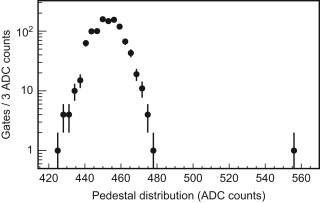
\includegraphics{Figures/Chapter2/Pedestal.jpg}
        \caption{Example of a pedestal distribution for a channel. In this case the the signal is above the normal pedestal distribution, this kind of gates are removed from the pedestal calculation. Figure from \cite{MINERvA}}
        \label{fig:MnvExp:MnvDetector:Calibration:InSitu:Pedestal}
    \end{figure}
    The pedestal subtraction, the mean pedestal is subtracted to the mean and remove the hits that do not pass the hit threshold.

    
    \item \textbf{PMT gain monitoring:} This consist in to inject light pulses (0.5 Hz) directly to the PMT using the LI system. This is turned on ones after each beam spill. This measurements are used to monitor the gain fluctuations of the PMTs. 
    
    The PMT gain is obtained using the data obtained when the LI system is turned on. The gain $g$ for a pixel is given by:

    \begin{equation}
        g=\frac{\Bar{Q}}{e\lambda},
        \label{eq:MnvExp:MnvDetector:Calibration:InSitu:Gain}
    \end{equation}
    where $\Bar{Q}$ is the mean of the anode charge distribution after the pedestal subtraction, $e$ is the electron charge and $\lambda$ is the average number of PEs arriving to the first dynode. The equation \ref{eq:MnvExp:MnvDetector:Calibration:InSitu:Gain} does not consider the effect due the quantum or collection efficiency of the PMT. The way that these parameters are included to gain calculation is assuming that the noise is well described by a Gaussian distribution and the dynode amplifies the charge following a Poison distribution can be obtained an expression that gives the gain as function of the variance of the noise and the variance of the distribution charge distribution.
    
    The average gain of a photomultipliers are normally  The variations in the gain measurement has a typical error of 1\%. 
    
    
    \item \textbf{Scintillator plane alignment:} The scintillator strips are held mechanically in the detector. During the assemble of the detector, small variations in the position of the planes or plastic strips. The calibration of the detector caused by the small variations uses the trajectory of the rock muons comparing the energy deposition on their points of intersection considering that each stripe has a base of 33 mm. 
    \begin{figure}[!htb]
        \centering
        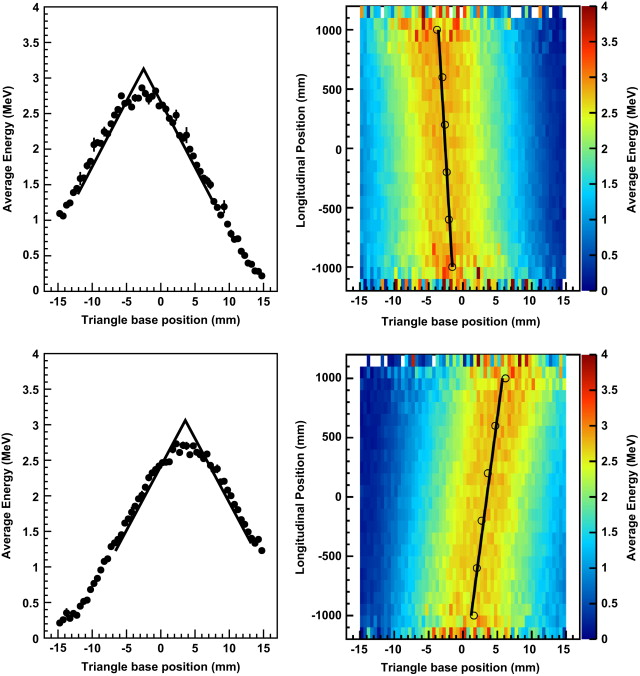
\includegraphics[scale=0.6]{Figures/Chapter2/AlignmentProfile.jpg}
        \caption{Image that shows two examples of alignment fits. The position respect to the XY axis is determined using average of the energy deposited in the strip, as is shown in  the left column. For the rotational parameter it depends of the shift in the longitudinal position.}
        \label{fig:MnvExp:MnvDetector:Calibration:InSitu:Alignment}
    \end{figure}
    Using the information of the deposited energy from the rock-muons in the plastic scintillators it is possible to measure the alignment in the XY plane and the rotational alignment respect to the Z axis. To measure the XY alignment is used the average deposited energy in the strip to determine the position of it respect the expected position. For the rotational position it can be given for the deposition of energy along to the strip for different rock-muon allowing a mapping of the strip, The \textbf{Figure} \ref{fig:MnvExp:MnvDetector:Calibration:InSitu:Alignment} shows an example of the alignment process. The precision of the alignment correction is 0.3 mm and 0.5 mrad on average.
    


    \item \textbf{Relative strip-to-strip response variations:} This calibration step is correlated to the effects of the variation between the scintillator strips, it could be for the fabrication imperfections of the couplings between the optical instrumentation. These variations are corrected by applying a correction factor to the deposited energy per strip. Normally these are obtained using the rock-muon data. 
    This procedure uses the truncated mean energy deposited per unit of length, after the average of the truncated mean energy is obtained for the hole plane. 

    The constant $C_i$\cite{MINERvA} for a strip $i$ is defined by:
    \begin{equation}
        C_i = \frac{\frac{1}{x_i}}{\frac{1}{N}\sum_j\frac{1}{x_j}}
        \label{eq:MnvExp:MnvDetector:Calibration:InSitu:ResponsStripConstant}
    \end{equation}

    where $x_i$ corresponds to the truncated mean energy in the strip $i$, N is the number of good channels and $j$ is the good channel index. 

    For the plane $j$, the constant $C^j$ \cite{MINERvA} is obtained by:

    \begin{equation}
        C^j = \frac{\frac{E^j}{p^j}}{\frac{1}{n}\sum_k\frac{E^k}{p^k}}
        \label{eq:MnvExp:MnvDetector:Calibration:InSitu:ResponsPlaneConstant}
    \end{equation}
    where $E^j$ is the average of the truncate mean energy for the plane $j$, $p^j$ is the fitted peak energy for a plane $j$, n is the number of planes and $k$ runs over all the planes.   
    
    Finally, the correction is made by multiplying the energy it by the constant found previously.   
    \item \textbf{Absolute energy scale determination:} Due the muon is a minimum ionizing particle ans it shows a well understood energy loos in plastic shintillator, it is used to determine an absolute energy scale called \textit{muon equivalent unit} (MEU). This factor is obtained by the use of the rock-muon data and simulation. 

    The rock-muons used have to pass throughout MINER$\nu$A and MINOS detectors, this with the aim to reconstruct the muon energy and momentum the best as possible. Giving as seed the momentum of the muon and the interaction position of the rock muon to the simulation it will produce a similar track. Then the clusters from the reconstruction in dta and simulation are compared. Using the information from data ans simulation the peak energy per unit of length is find. The MEU factor is obtained multiplying the previous MEU factor by the ratio of the peaks of the reconstructed cluster energy distributions ($\frac{E_{sim}}{E_{Data}}$), divided by the efficiency of the reconstructed energy in the simulation.

    This calibration allows to have an agreement between the data and simulation energy reconstruction of PEs. The usual value of this MEU factor is 0.08 MeV/PE.
    \item \textbf{Timing calibration:} This calibration step consists in the correction of the time offsets. Th time offsets are produced mainly for the following reasons:
    \begin{itemize}
        \item The transport of the light from the plastic scintillator to the PMT.
        \item The processing time required by the electronics tho process the signal and sent it along the cables and the chain.  
        \item The \textit{time slewing}, it is correlated to the time that take to the scintillator decays.
    \end{itemize}

    The calibration is made using the rock-muon's track information. For this the average time-of-flight of the muon is calculated and the hit time along to the muon track is compared with it as reference, obtaining the in this way the total offset. The next step is to find the time slewing which is find as function of the PE, the \textbf{Figure} \ref{fig:MnvExp:MnvDetector:Calibration:InSitu:SlewingFunc} shows the measured time slewing example. The offset due the transport of light is estimated considering the light velocity in the materials and the lengths of the fibers. The time offset for the electronics is calculated using the difference between the reference muon track and the hit time.  
    \begin{figure}[!htb]
        \centering
        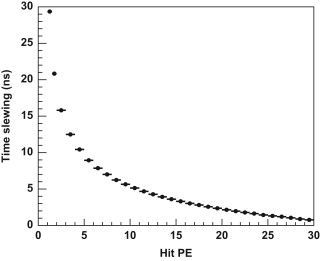
\includegraphics{Figures/Chapter2/SlewingFunction.jpg}
        \caption{Plot with the time slewing as function of the hit PE for a single strip. Figure from \cite{MINERvA}}
        \label{fig:MnvExp:MnvDetector:Calibration:InSitu:SlewingFunc}
    \end{figure}
    \item \textbf{Cross-talk:} Cross-talk occurs when light arriving at one PMT produces a signal in another channel that does not correspond to the actual channel. The typical reasons for cross-talk in MINER$\nu$A are related to the fibers to PMT coupling or PMT internal dynodes chain imperfections.

    To characterize the  signals produced by cross-talk the signals obtained from rock muons are used. The way that the optical fibers are arranged in to the PMTs produce that the signals produced by the cross-talk corresponds to channels that are far from the particle trajectory. The signal produced by the cross-talk channels is very characteristic at difference to other noise sources because these are produced at the same time that the muon track signal.

    \begin{figure}[!htb]
        \centering
        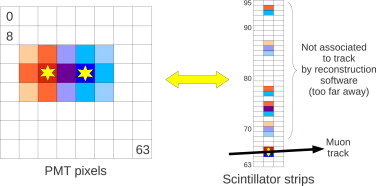
\includegraphics{Figures/Chapter2/CrossTallkExample.jpg}
        \caption{An example illustrates how cross-talk manifests in a muon trajectory and demonstrates the process of removing hits that do not correspond to the muon track. Figure from \cite{MINERvA}}
        \label{fig:Chapter2:CrossTallkExample}
    \end{figure}
    After to identify the muon-track hits and the cross-talk, $f_{xt,NN}$ is defined as the ratio between muon-track and cross-talk energy hits. This metric is used to determine the \textit{nearest neighbor} pixel cross-talk. This quantity usually is below the 4\%. This quantity is usually used to compare the simulated cross-talk, this information is used to have a more accurate simulation of the detector.  
    
\end{itemize}

\pagebreak


\subsection{Data Reconstruction}
\label{Cap:MnvExp:MnvDetector:DataReconstruction}

After calibrating the data, the next step is to reconstruct the events. It consists of using the energy hits to reconstruct the trajectories, energy, momentum, and hypothesize about the particle identification. 

\subsubsection{Time Slicing}
\label{Cap:MnvExp:MnvDetector:DataReconstruction:TimeSlicing}

In a gate, multiple neutrino events can be produced. To separate the different interactions in a gate, an algorithm \textit{ slicer} separates the activity of the detector into groups. This group does not need to have spatial relation, these groups are called \textit{time slices}. The duration of this time slices are typically below 100 ns with a minimum of 80 ns for the LE era; for the ME era it decreases the minimum to 24 ns due to the intensity increase of the neutrino beam. Typically a time slice contains only one neutrino event, with the exception of the michel electrons that are produced by the decay of stooped muons in the detector, these are observed some time slices after the interaction. The \textbf{Figure} \ref{fig:MnvExp:MnvDetector:CalibrationOneGate} shows a gate on how it separates events by time slices.

\begin{figure}[!htb]
    \centering
    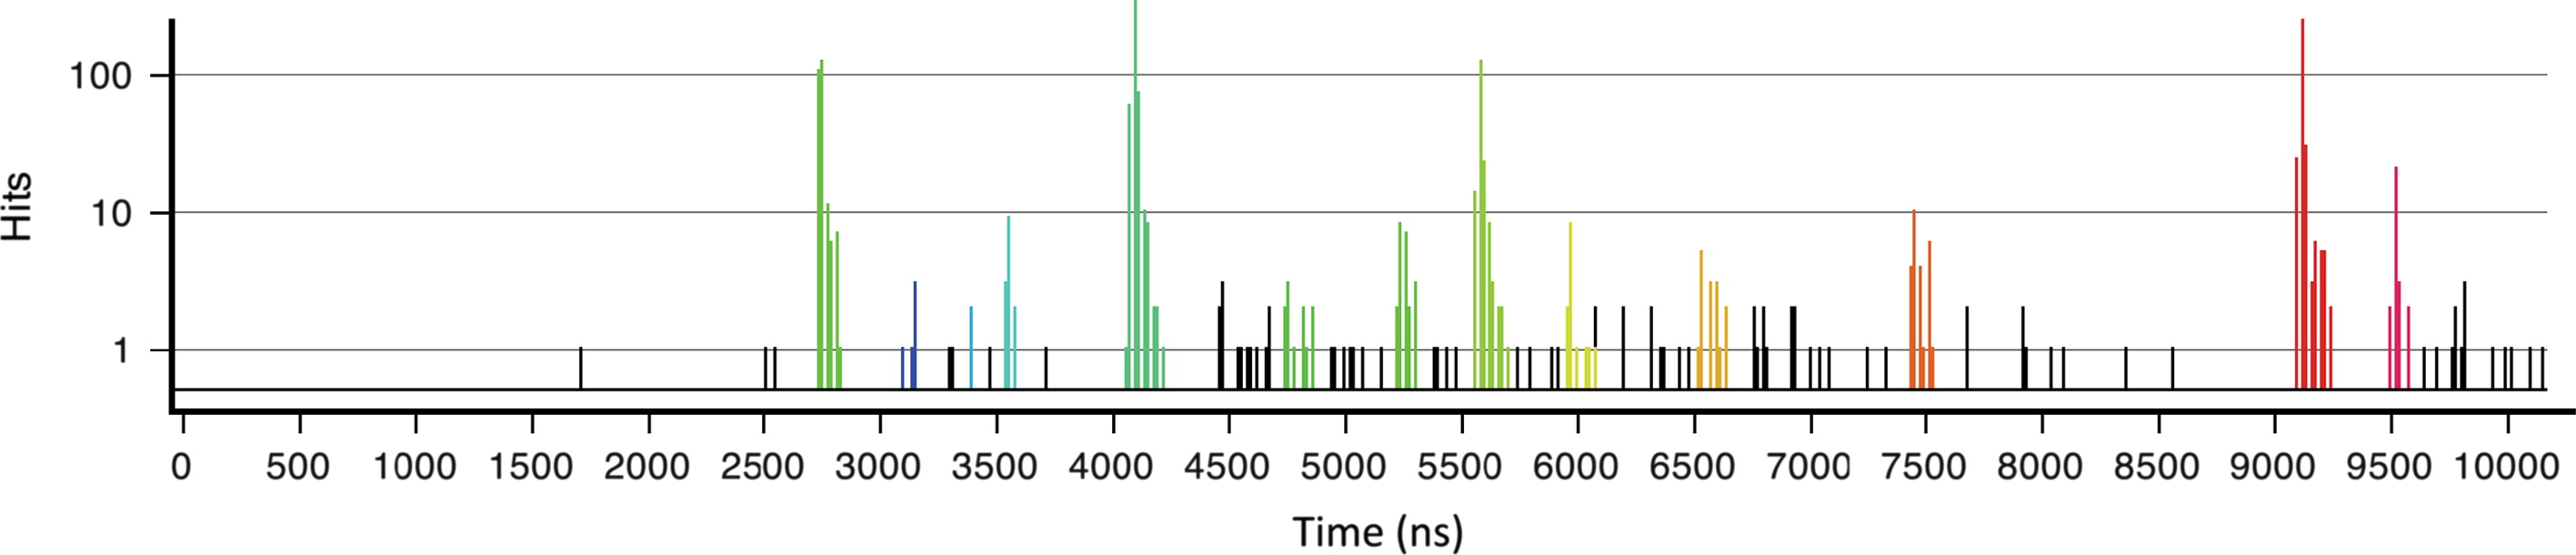
\includegraphics[scale=1]{Figures/Chapter2/OneGate.jpg}
    \caption{Image that shows activity in the detector for a readout gate. In the image the colored groups of activity are represents a time slice. Figure taken from \cite{MINERvA}}
    \label{fig:MnvExp:MnvDetector:CalibrationOneGate}
\end{figure}
The slicer looks for groups of hits continues on time where the sum of the hits energy passes the threshold for 10 PE, fixing a time slice. The slicer also consider the time uncertainties that can be produced by a miss-calibration, explained in the previous subsection. Considering this, after that the time slicer is have been set, the slicer looks for hits at 9 ns from the limits if it founds more hits these are included in the time slice and the process is made again until it does not find events above the 9 ns in the edges. 

\subsubsection{Muon Reconstruction}
\label{Cap:MnvExp:MnvDetector:DataReconstruction:MuonReconstruction}
In MINER$\nu$A, muon reconstruction entails reconstructing the muon track in the MINOS Near detector. To achieve a comprehensive reconstruction, the muon must first be detected in the MINER$\nu$A detector and then observed in MINOS. The time window during which the muon is detected in MINER$\nu$A must align with the arrival time of a muon at the MINOS detector, with a time difference permitted of approximately $\pm50$ ns for an event to be considered a match. In addition, the spatial alignment of the tracks is also required. 

The momentum of the muon is reconstructed in MINOS using range or curvature techniques. For this analysis, it is also important to know the direction of the curvature of the muon track in MINOS because it gives information about the charge signal of the muon. The charge signal is used to determine whether the interaction was due to a neutrino or antineutrino Charged Current interaction.

For muons contained within the detector, the muon momentum is reconstructed using the range method. This involves utilizing the Bethe-Bloch equation to estimate the energy deposited by the muon in the plastic scintillator and the steel layers within the detector. The uncertainty associated with the range-based reconstruction is 0.98\%. 

For the cases where the muon momentum is reconstructed curvature, the momentum is calculated as follows:

\begin{equation}
    p = 0.3\times B \times q_\mu \times R,
\end{equation}

where $B$ is the magnetic field magnitude, $q_\mu$ is the muon charge, and $R$ is the radio of the curvature. The uncertainty associated with the reconstruction of the curvature is between 0. 6\% and 2. 5\%. 



\subsubsection{Clustering}
\label{Cap:MnvExp:MnvDetector:DataReconstruction:Clustering}

The time slices groups looking for hits continues in the time to produce the time slices, the next step is to do the same but looking for hist continuous in the space for the same time slice. These hits groups are called \textit{ clusters}. The clusters use the information from the hits to measure the energy by summing the hits energy of all the groups. If there is a cluster that is not connected with the other clusters by other hits in the same time slice, these are called isolated clusters.

\begin{figure}[!htb]
    \centering
    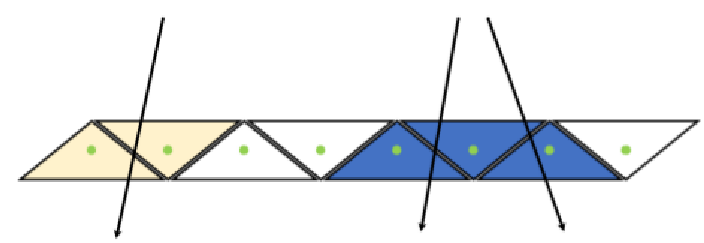
\includegraphics[scale=0.5]{Figures/Chapter2/ClusterFormation.png}
    \caption{The design of the planes makes that the particles that pass throughout a plane must to produce signal in at least 2 scintillator strips. Figure from \cite{AaronThesis}.}
    \label{fig:MnvExp:MnvDetector:DataReconstruction:Clustering:ClusterFormation}
\end{figure}

Each cluster is tagged using the time information and the deposited energy in the strips. Depending on the composition of the cluster, these are classified as low activity, trackable, heavily ionizing, superclusters, or cross-talk. The classes are described in the \textbf{Table} \ref{tab:MnvExp:MnvDetector:DataReconstruction:Clustering:ClusterClasses} and the \textbf{Figure} \ref{fig:MnvExp:MnvDetector:DataReconstruction:Clustering:ClusterSketch} shows some examples of how these are observed in the planes.

\begin{table}[!htb]
    \centering
    \begin{tabular}{c|p{3.5in}}
        Classification & Description \\ \hline
        Low activity & Cluster with a total energy below 1 MeV\\ \hline
        Trackeabke & Cluster with a total energy between 1-12 MeV and between 1-3 hits with at least one hit with 0.5 MeV of energy. Multiple hits with 0.5 MeV must be adjacent.\\ \hline
        Heavily ionizing & Cluster with a total energy $>$ 1 MeV with 1-3 hist with an energy > 0.5 MeV. The hits with energy above 0.5 MeV must be adjacent to each other. \\ \hline
        Superclusters & The total energy of the cluster is above 1 MeV, more than 4 hits, and the multiple hits with energy above 0.5 MeV do not need to be adjacent. \\ \hline
        Cross-talk & These are identified by understanding the mapping of the PMT pixels. They are spatially distant from the other hits and usually have low energy.\\ \hline
    \end{tabular}
    \caption{Cluster classification and short description of them.}
    \label{tab:MnvExp:MnvDetector:DataReconstruction:Clustering:ClusterClasses}
\end{table}



\begin{figure} [!htb]
    \centering
    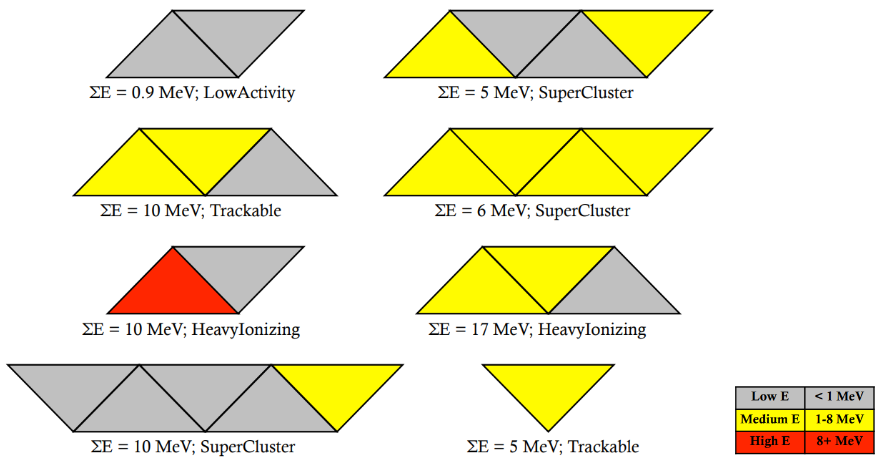
\includegraphics[scale=0.5]{Figures/Chapter2/ClusterScketch.png}
    \caption{Sketch that show how are observed the different cluster classes. Figure taken from \cite{PerduePresentation}.}
    \label{fig:MnvExp:MnvDetector:DataReconstruction:Clustering:ClusterSketch}
\end{figure}

\subsubsection{Track Reconstruction}
\label{Cap:MnvExp:MnvDetector:DataReconstruction:TrackReconstruction}

The cluster information is used to build an object called \textit{track}. This object approximates a 3D trajectory of the particles passing throughout the detector. The algorithms used to reconstruct the tracks of the particles are called \textit{trackers}. There are different algorithms that create these objects and can be categorized in two types. The long and short trackers. 

The long tracker algorithm uses only the trackable and heavy ionizing clusters. The long tracker needs at least 9 planes long and angles below 60 degrees to reconstruct the track. The clusters are grouped in the same plane view (X, U, V) to track the \textit{ seedlings}. Each seed is used to determine a 2D line by a fit of $\chi^2$. The track seeds can share clusters with other seeds. The seeds that share at least one cluster are then merged to give a candidate track. Finally, the tracks candidates are used to reconstruct a 3D track. In this step, the super clusters are added to the track reconstruction. For the tracks that are close to the estimated vertex, the Kalman filter technique \cite{KalmanFilter} is used to reestimate the vertex position using the information of all the tracks. The last step also cleans the track, removing the hits from the super-clusters that do not correspond to the track of the particle and creating new clusters. The \textbf{Figure} \ref{fig:MnvExp:MnvDetector:DataReconstruction:LongTrackreconstruction} shows the steps to follow to make a track reconstruction. 

\begin{figure}[!htb]
    \centering
    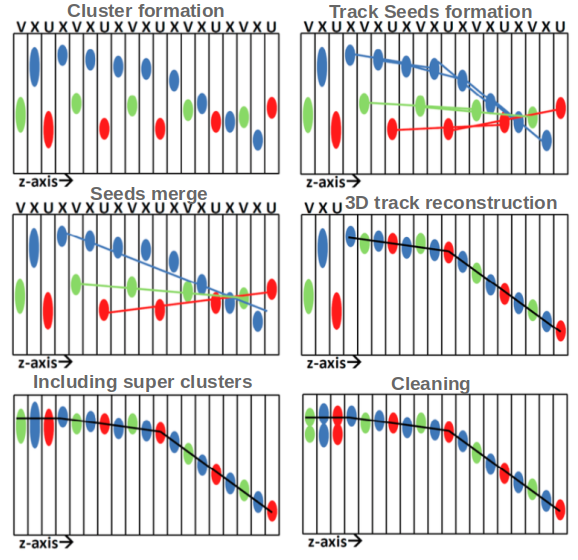
\includegraphics[scale=0.5]{Figures/Chapter2/LongTracking.png}
    \caption{Sketch that shows the different steps followed by the long track algorithm to reconstruct the 3D trajectory of particles.}\label{fig:MnvExp:MnvDetector:DataReconstruction:LongTrackreconstruction}
\end{figure}

The short tracker algorithm is capable to reconstruct particle trajectories with at least five planes. The distance of 5 planes corresponds to 6.8 cm, measured from the center of a triangular strip. This distance corresponds to the energy deposited by a pion with a kinetic energy of 35 MeV. The short tracker uses the continuous clusters and for at least two seeds to produce a 3D track. Similarly to the long tracker, the seeds are merged to produce the 3D track candidate. For a detailed description of long and short trackers \cite{AaronThesis}.

The long tracker identifies the longest track and designates it as an anchor track. It assumes that the particle trajectory is directed downstream towards the MINOS detector, with the vertex position set at the track end located upstream of the detector. Generally, the long track corresponds to the lepton track, regularly to a muon, this track is also called a \textit{primary} track.

After setting the vertex, the next step is to search for other tracks consistent with its position. For this step, all tracks found using the short or long track algorithms are considered. They must satisfy the condition that their nearest cluster to the vertex is at most 250 mm away, and the track projection in the XY plane is at most 100 mm from the vertex. Tracks meeting these criteria are designated as primary or anchor tracks.  

The final step is to find the secondary tracks. These tracks can be produced by a nonionizing interaction of the particles with the detector, these interactions produce a drastic change of the trajectory of the particles or the creation of more particles. The secondary particles are found checking the clusters in the end of the primary clusters and the upstream cluster of the secondary particle; if the secondary track is consistent with the distance criteria described for the primary vertex, it is considered as a secondary particle. 


\subsubsection{Hadronic Recoil Energy Reconstruction}
\label{Cap:MnvExp:MnvDetector:DataReconstruction:ENergyReconstruction}

The hadronic recoil energy is essential to measure variables such as the invariant mass ($W_{exp}$), Four-momentum transfer ($Q^2$), or the neutrino energy.

To completely reconstruct the hadronic energy ($E_{had}$) it is necessary to know the energy of all non-muon particles produced in the interaction vertex. Unfortunately, the neutral particles do not produce a visible track in the detector ant it is not possible to detect them directly. The energy estimation for neutral particles such as neutrons or neutral pions is made using the particles produced in their decay. 

\begin{figure}[!htb]
    \centering
    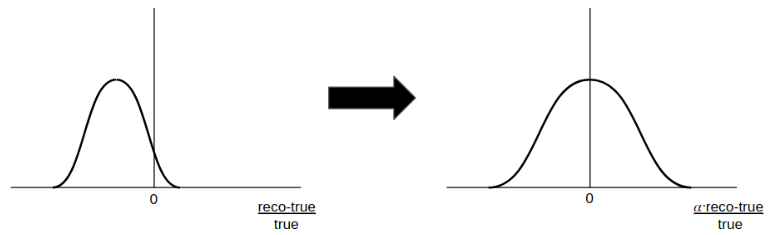
\includegraphics[scale=0.5]{Figures/Chapter2/CorrectionFactor.png}
    \caption{In the left is the resolution distribution without correction is showed. The right distribution shows how the correction factor shifts the distribution centering it in zero. Figure from \cite{AaronThesis}.}
    \label{fig:MnvExp:MnvDetector:DataReconstruction:EnergyRes}
\end{figure}

The hadronic recoil energy is reconstructed summing the energy from the nonmuon cluster energy. Next, the summed energy is adjusted by the calorimetric correction which is used to compensate the not observed energy. To obtain the correction, multiple events are simulated in the detector materials to measure the energy of the particles that are visible and then to find the bias between the visible ($E_{vis}$) and the truth energy ($E_{true}$) calculating the energy resolution $\frac{E_{vis} - E_{true}}{E_{true}}$. The distribution obtained can be fitted by a Gaussian distribution with the center shifted from zero. The correction factor displaces the Gaussian distribution center to the cero. This correction is highly dependent on the model. The uncertainties related to these corrections are added to the cross section calculation. 

    \subsubsection{Michel Electron Reconstruction}
\label{Cap:MnvExp:MnvDetector:DataReconstruction:MichelElectron}

The michel electrons are observed in the detector when a stooped muon decays in the detector and produces two neutrinos and an electron or positron, depending on the initial muon charge. The detection of the michel electrons is essential for analysis, where a charge pion is needed. For example, in this analysis it is used to apply cuts during the data selection and to estimate the kinetic energy of the pion, for more information check \ref{Cap:Analysis:DataSelection:Cuts} and \ref{Cap:MnvExp:MnvDetector:DataReconstruction:Untrackedpions}. 

The michel electrons are found time slices after the interaction, it is because the mean lifetime of the muon is ($\tau_\mu$) 2.2 $\mu$s. The mean life time of the pion ($\tau_\pi$ = 26 ns) is not really relevant to be considered in the calculation of the time to observe the michel electron. From the pion decay, most part of the energy is transferred to the neutrino, therefore the muon only deposits around 4 MeV of visible energy in the detector. Due to the deadtime \cite{MINERvA} of the detector the energy of the muon is not recorded, allowing to observe a clear time delay between the interaction slice and the michel electron slice. 

The michel electron slice must to meet the following conditions to be considered as a michel electron candidate:
\begin{itemize}
    \item Energy consistent to the three body decay of a muon, in the MINER$\nu$A detector it is between 10 and 65 MeV. 
    \item The time slice must be between $\pm$ 25 gaps for the energy-weighted time average. 
    \item The distance between the cluster and the energy weighted longitudinal position must be below 35 cm. 
\end{itemize}

The \textbf{Figure}\ref{fig:Analysis:DataSelection:Cuts:Tracked:EventDisplayMETracked} shows a simulated signal event where the michel electron is shown after 4 slices. 

\subsubsection{Untracked pions Reconstruction}
\label{Cap:MnvExp:MnvDetector:DataReconstruction:Untrackedpions}

As explained in the previous subsection, the michel electron can be used to find events where pions are produced. This section explains a new technique that allows one to estimate the kinetic energy and the angle respect to the beam of events where charge pions are produced without the requirement to reconstruct the pion track. This reconstruction allows to remove low threshold for the pion kinetic energy in this analysis.
 
The first step is to identify the fitted Michel electron candidates. A Michel electron candidate falls into the fitted category when it passes through multiple planes and a fitted line can be found that passes through the Michel candidate clusters. For a detailed description of the adjustment procedure, refer to \cite{AaronThesis}. The fitted line enables the definition of the end point positions, with each end point indexed based on its location being more downstream in the detector.

After finding the michel electron candidate endpoints, the next step is to obtain 3D distance between the endpoints and the reconstructed vertex position, selecting the closest endpoint. The distance between the closest endpoint and the vertex is called the \textit{pion range}. 

\begin{figure}
    \centering
    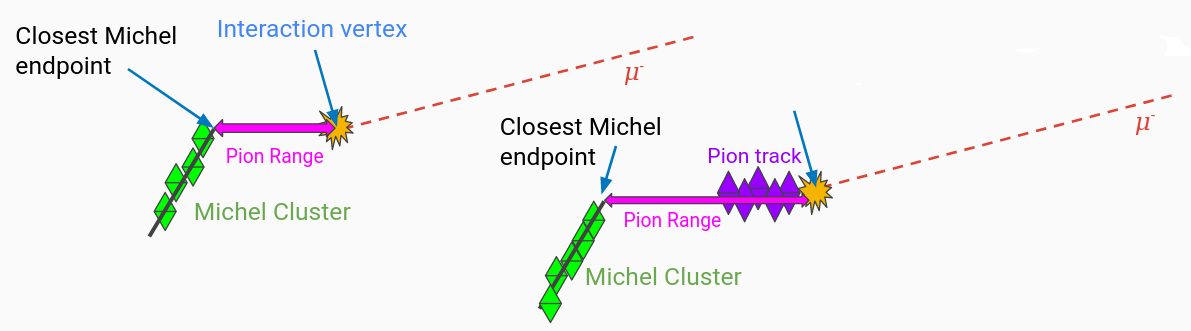
\includegraphics[scale=0.33]{Figures/Chapter4/DataSelection/TracklessPions.png}
    \caption{Scheme that shows how is measured the pion range for an event with a michel electron. }
    \label{fig:MnvExp:MnvDetector:DataReconstruction:UntrackedpionsMichelEventSheme}
\end{figure}


Next, using simulated data, a 2D histogram with the reconstructed pion range and the simulated pion kinetic energy in the final state for events with at least one fitted michel electron is used to produce a singular dot getting the bin center of the bin with the maximum value for each bin of the pion range, in the \textbf{Figure} \ref{fig:MnvExp:MnvDetector:DataReconstruction:Untrackedpions:TpivsPionRange} the 2D histogram is shown.

\begin{figure}[!htb]
    \centering
    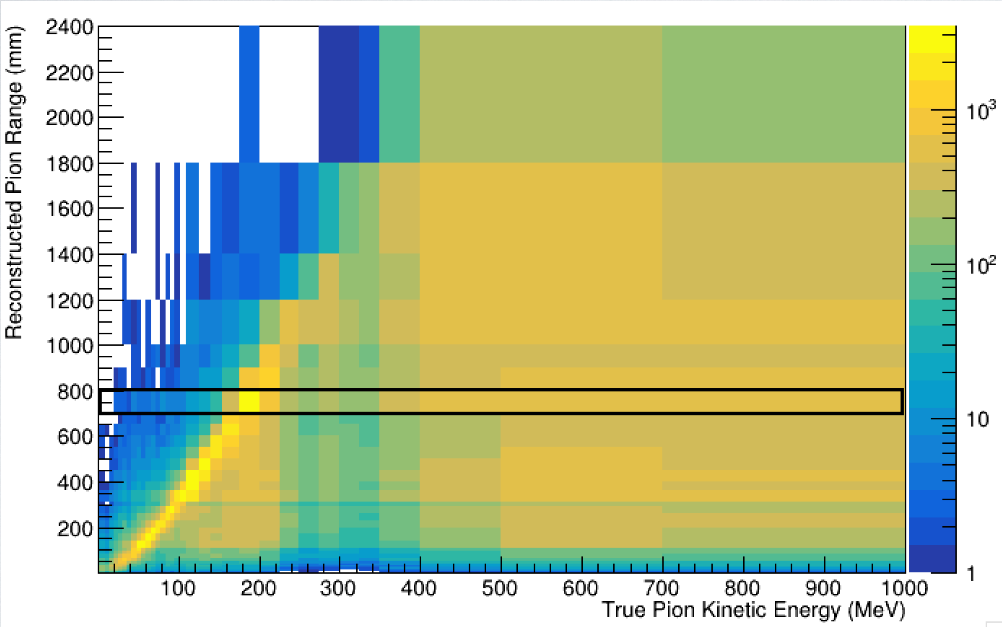
\includegraphics[scale=0.33]{Figures/Chapter2/TpivsPionRange.png}
    \caption{Bin normalized 2D histogram with the true pion kinetic energy (Y axis) and the reconstructed pion (X axis). This histogram is subdivided on bins of pion range as is observed in the figure to obtain the bin with the maximum value as function of the kinetic energy. }
    \label{fig:MnvExp:MnvDetector:DataReconstruction:Untrackedpions:TpivsPionRange}
\end{figure}

After getting the points where there are more coincidences of the kinetic energy as a function of the pion range these points are used to fit a function in the way that a relation is obtained between the true pion kinetic energy and the pion range. The function fitted is:

\begin{equation}
    T_{\pi^+} = p_0 x+p_1 \sqrt{x}
\end{equation}

where $p_0$ and $p_1$ are two free parameters that will be fitted and $x$ is the pion range. The \textbf{Figure} \ref{fig:MnvExp:MnvDetector:DataReconstruction:Untrackedpions:PionEstimator} shows the fitting result with the point obtained from the histogram in the \textbf{Figure} \ref{fig:MnvExp:MnvDetector:DataReconstruction:Untrackedpions:TpivsPionRange}.

\begin{figure}[!htb]
    \centering
    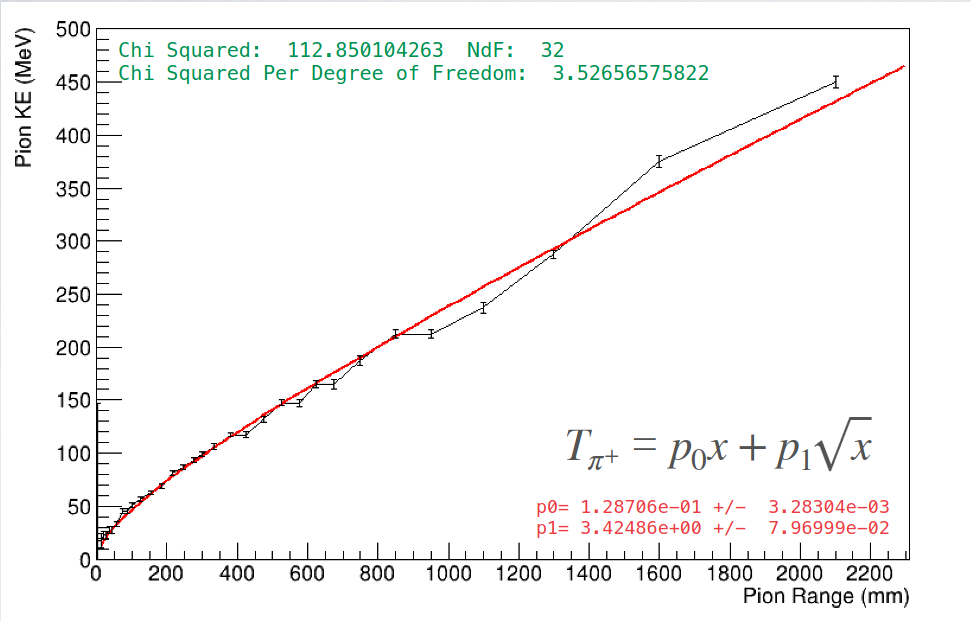
\includegraphics[scale=0.33]{Figures/Chapter2/PionEstimator.png}
    \caption{Scheme that shows how is measured the pion range for an event with a michel electron. }
    \label{fig:MnvExp:MnvDetector:DataReconstruction:Untrackedpions:PionEstimator}
\end{figure}

The final relation used to estimate the pion kinetic energy is:
\begin{equation}
    T_{\pi^+} = 0.128706 x+ 3.42486 \sqrt{x}
\end{equation}

The estimation of the pion angle is determined by the position of the closest Michel electron endpoint. The angle obtained represents the angle between the neutrino beam direction and a line passing through the vertex and the endpoint position. 
